\documentclass[twoside]{book}

% Packages required by doxygen
\usepackage{fixltx2e}
\usepackage{calc}
\usepackage{doxygen}
\usepackage[export]{adjustbox} % also loads graphicx
\usepackage{graphicx}
\usepackage[utf8]{inputenc}
\usepackage{makeidx}
\usepackage{multicol}
\usepackage{multirow}
\PassOptionsToPackage{warn}{textcomp}
\usepackage{textcomp}
\usepackage[nointegrals]{wasysym}
\usepackage[table]{xcolor}

% Font selection
\usepackage[T1]{fontenc}
\usepackage[scaled=.90]{helvet}
\usepackage{courier}
\usepackage{amssymb}
\usepackage{sectsty}
\renewcommand{\familydefault}{\sfdefault}
\allsectionsfont{%
  \fontseries{bc}\selectfont%
  \color{darkgray}%
}
\renewcommand{\DoxyLabelFont}{%
  \fontseries{bc}\selectfont%
  \color{darkgray}%
}
\newcommand{\+}{\discretionary{\mbox{\scriptsize$\hookleftarrow$}}{}{}}

% Page & text layout
\usepackage{geometry}
\geometry{%
  a4paper,%
  top=2.5cm,%
  bottom=2.5cm,%
  left=2.5cm,%
  right=2.5cm%
}
\tolerance=750
\hfuzz=15pt
\hbadness=750
\setlength{\emergencystretch}{15pt}
\setlength{\parindent}{0cm}
\setlength{\parskip}{3ex plus 2ex minus 2ex}
\makeatletter
\renewcommand{\paragraph}{%
  \@startsection{paragraph}{4}{0ex}{-1.0ex}{1.0ex}{%
    \normalfont\normalsize\bfseries\SS@parafont%
  }%
}
\renewcommand{\subparagraph}{%
  \@startsection{subparagraph}{5}{0ex}{-1.0ex}{1.0ex}{%
    \normalfont\normalsize\bfseries\SS@subparafont%
  }%
}
\makeatother

% Headers & footers
\usepackage{fancyhdr}
\pagestyle{fancyplain}
\fancyhead[LE]{\fancyplain{}{\bfseries\thepage}}
\fancyhead[CE]{\fancyplain{}{}}
\fancyhead[RE]{\fancyplain{}{\bfseries\leftmark}}
\fancyhead[LO]{\fancyplain{}{\bfseries\rightmark}}
\fancyhead[CO]{\fancyplain{}{}}
\fancyhead[RO]{\fancyplain{}{\bfseries\thepage}}
\fancyfoot[LE]{\fancyplain{}{}}
\fancyfoot[CE]{\fancyplain{}{}}
\fancyfoot[RE]{\fancyplain{}{\bfseries\scriptsize Generated by Doxygen }}
\fancyfoot[LO]{\fancyplain{}{\bfseries\scriptsize Generated by Doxygen }}
\fancyfoot[CO]{\fancyplain{}{}}
\fancyfoot[RO]{\fancyplain{}{}}
\renewcommand{\footrulewidth}{0.4pt}
\renewcommand{\chaptermark}[1]{%
  \markboth{#1}{}%
}
\renewcommand{\sectionmark}[1]{%
  \markright{\thesection\ #1}%
}

% Indices & bibliography
\usepackage{natbib}
\usepackage[titles]{tocloft}
\setcounter{tocdepth}{3}
\setcounter{secnumdepth}{5}
\makeindex

% Hyperlinks (required, but should be loaded last)
\usepackage{ifpdf}
\ifpdf
  \usepackage[pdftex,pagebackref=true]{hyperref}
\else
  \usepackage[ps2pdf,pagebackref=true]{hyperref}
\fi
\hypersetup{%
  colorlinks=true,%
  linkcolor=blue,%
  citecolor=blue,%
  unicode%
}

% Custom commands
\newcommand{\clearemptydoublepage}{%
  \newpage{\pagestyle{empty}\cleardoublepage}%
}

\usepackage{caption}
\captionsetup{labelsep=space,justification=centering,font={bf},singlelinecheck=off,skip=4pt,position=top}

%===== C O N T E N T S =====

\begin{document}

% Titlepage & ToC
\hypersetup{pageanchor=false,
             bookmarksnumbered=true,
             pdfencoding=unicode
            }
\pagenumbering{alph}
\begin{titlepage}
\vspace*{7cm}
\begin{center}%
{\Large My Project }\\
\vspace*{1cm}
{\large Generated by Doxygen 1.8.12}\\
\end{center}
\end{titlepage}
\clearemptydoublepage
\pagenumbering{roman}
\tableofcontents
\clearemptydoublepage
\pagenumbering{arabic}
\hypersetup{pageanchor=true}

%--- Begin generated contents ---
\chapter{Deprecated List}
\label{deprecated}
\hypertarget{deprecated}{}

\begin{DoxyRefList}
\item[\label{deprecated__deprecated000001}%
\hypertarget{deprecated__deprecated000001}{}%
Member \hyperlink{classorg_1_1elasticsearch_1_1_exceptions_helper_a9ceadc9e3e73578bcf5ad6f14c91e6ff}{org.elasticsearch.Exceptions\+Helper.detailed\+Message} (Throwable t)]Don\textquotesingle{}t swallow exceptions, allow them to propagate. 
\end{DoxyRefList}
\chapter{Namespace Index}
\section{Packages}
Here are the packages with brief descriptions (if available)\+:\begin{DoxyCompactList}
\item\contentsline{section}{\hyperlink{namespaceorg_1_1elasticsearch}{org.\+elasticsearch} }{\pageref{namespaceorg_1_1elasticsearch}}{}
\end{DoxyCompactList}

\chapter{Hierarchical Index}
\section{Class Hierarchy}
This inheritance list is sorted roughly, but not completely, alphabetically\+:\begin{DoxyCompactList}
\item \contentsline{section}{org.\+elasticsearch.\+Build}{\pageref{classorg_1_1elasticsearch_1_1_build}}{}
\item \contentsline{section}{org.\+elasticsearch.\+Elasticsearch\+Wrapper\+Exception}{\pageref{interfaceorg_1_1elasticsearch_1_1_elasticsearch_wrapper_exception}}{}
\item \contentsline{section}{org.\+elasticsearch.\+Exceptions\+Helper}{\pageref{classorg_1_1elasticsearch_1_1_exceptions_helper}}{}
\item Runtime\+Exception\begin{DoxyCompactList}
\item \contentsline{section}{org.\+elasticsearch.\+Elasticsearch\+Exception}{\pageref{classorg_1_1elasticsearch_1_1_elasticsearch_exception}}{}
\begin{DoxyCompactList}
\item \contentsline{section}{org.\+elasticsearch.\+Elasticsearch\+Generation\+Exception}{\pageref{classorg_1_1elasticsearch_1_1_elasticsearch_generation_exception}}{}
\item \contentsline{section}{org.\+elasticsearch.\+Elasticsearch\+Parse\+Exception}{\pageref{classorg_1_1elasticsearch_1_1_elasticsearch_parse_exception}}{}
\item \contentsline{section}{org.\+elasticsearch.\+Elasticsearch\+Status\+Exception}{\pageref{classorg_1_1elasticsearch_1_1_elasticsearch_status_exception}}{}
\begin{DoxyCompactList}
\item \contentsline{section}{org.\+elasticsearch.\+Elasticsearch\+Security\+Exception}{\pageref{classorg_1_1elasticsearch_1_1_elasticsearch_security_exception}}{}
\end{DoxyCompactList}
\item \contentsline{section}{org.\+elasticsearch.\+Elasticsearch\+Timeout\+Exception}{\pageref{classorg_1_1elasticsearch_1_1_elasticsearch_timeout_exception}}{}
\item \contentsline{section}{org.\+elasticsearch.\+Resource\+Not\+Found\+Exception}{\pageref{classorg_1_1elasticsearch_1_1_resource_not_found_exception}}{}
\end{DoxyCompactList}
\end{DoxyCompactList}
\item \contentsline{section}{org.\+elasticsearch.\+Version}{\pageref{classorg_1_1elasticsearch_1_1_version}}{}
\item Basic\+Permission\begin{DoxyCompactList}
\item \contentsline{section}{org.\+elasticsearch.\+Special\+Permission}{\pageref{classorg_1_1elasticsearch_1_1_special_permission}}{}
\end{DoxyCompactList}
\item I\+O\+Exception\begin{DoxyCompactList}
\item \contentsline{section}{org.\+elasticsearch.\+Elasticsearch\+Corruption\+Exception}{\pageref{classorg_1_1elasticsearch_1_1_elasticsearch_corruption_exception}}{}
\end{DoxyCompactList}
\item To\+X\+Content\begin{DoxyCompactList}
\item \contentsline{section}{org.\+elasticsearch.\+Elasticsearch\+Exception}{\pageref{classorg_1_1elasticsearch_1_1_elasticsearch_exception}}{}
\end{DoxyCompactList}
\item Writeable\begin{DoxyCompactList}
\item \contentsline{section}{org.\+elasticsearch.\+Elasticsearch\+Exception}{\pageref{classorg_1_1elasticsearch_1_1_elasticsearch_exception}}{}
\end{DoxyCompactList}
\end{DoxyCompactList}

\chapter{Class Index}
\section{Class List}
Here are the classes, structs, unions and interfaces with brief descriptions\+:\begin{DoxyCompactList}
\item\contentsline{section}{\hyperlink{classorg_1_1elasticsearch_1_1_build}{org.\+elasticsearch.\+Build} }{\pageref{classorg_1_1elasticsearch_1_1_build}}{}
\item\contentsline{section}{\hyperlink{classorg_1_1elasticsearch_1_1_elasticsearch_corruption_exception}{org.\+elasticsearch.\+Elasticsearch\+Corruption\+Exception} }{\pageref{classorg_1_1elasticsearch_1_1_elasticsearch_corruption_exception}}{}
\item\contentsline{section}{\hyperlink{classorg_1_1elasticsearch_1_1_elasticsearch_exception}{org.\+elasticsearch.\+Elasticsearch\+Exception} }{\pageref{classorg_1_1elasticsearch_1_1_elasticsearch_exception}}{}
\item\contentsline{section}{\hyperlink{classorg_1_1elasticsearch_1_1_elasticsearch_generation_exception}{org.\+elasticsearch.\+Elasticsearch\+Generation\+Exception} }{\pageref{classorg_1_1elasticsearch_1_1_elasticsearch_generation_exception}}{}
\item\contentsline{section}{\hyperlink{classorg_1_1elasticsearch_1_1_elasticsearch_parse_exception}{org.\+elasticsearch.\+Elasticsearch\+Parse\+Exception} }{\pageref{classorg_1_1elasticsearch_1_1_elasticsearch_parse_exception}}{}
\item\contentsline{section}{\hyperlink{classorg_1_1elasticsearch_1_1_elasticsearch_security_exception}{org.\+elasticsearch.\+Elasticsearch\+Security\+Exception} }{\pageref{classorg_1_1elasticsearch_1_1_elasticsearch_security_exception}}{}
\item\contentsline{section}{\hyperlink{classorg_1_1elasticsearch_1_1_elasticsearch_status_exception}{org.\+elasticsearch.\+Elasticsearch\+Status\+Exception} }{\pageref{classorg_1_1elasticsearch_1_1_elasticsearch_status_exception}}{}
\item\contentsline{section}{\hyperlink{classorg_1_1elasticsearch_1_1_elasticsearch_timeout_exception}{org.\+elasticsearch.\+Elasticsearch\+Timeout\+Exception} }{\pageref{classorg_1_1elasticsearch_1_1_elasticsearch_timeout_exception}}{}
\item\contentsline{section}{\hyperlink{interfaceorg_1_1elasticsearch_1_1_elasticsearch_wrapper_exception}{org.\+elasticsearch.\+Elasticsearch\+Wrapper\+Exception} }{\pageref{interfaceorg_1_1elasticsearch_1_1_elasticsearch_wrapper_exception}}{}
\item\contentsline{section}{\hyperlink{classorg_1_1elasticsearch_1_1_exceptions_helper}{org.\+elasticsearch.\+Exceptions\+Helper} }{\pageref{classorg_1_1elasticsearch_1_1_exceptions_helper}}{}
\item\contentsline{section}{\hyperlink{classorg_1_1elasticsearch_1_1_resource_not_found_exception}{org.\+elasticsearch.\+Resource\+Not\+Found\+Exception} }{\pageref{classorg_1_1elasticsearch_1_1_resource_not_found_exception}}{}
\item\contentsline{section}{\hyperlink{classorg_1_1elasticsearch_1_1_special_permission}{org.\+elasticsearch.\+Special\+Permission} }{\pageref{classorg_1_1elasticsearch_1_1_special_permission}}{}
\item\contentsline{section}{\hyperlink{classorg_1_1elasticsearch_1_1_version}{org.\+elasticsearch.\+Version} }{\pageref{classorg_1_1elasticsearch_1_1_version}}{}
\end{DoxyCompactList}

\chapter{Namespace Documentation}
\hypertarget{namespaceorg_1_1elasticsearch}{}\section{Package org.\+elasticsearch}
\label{namespaceorg_1_1elasticsearch}\index{org.\+elasticsearch@{org.\+elasticsearch}}
\subsection*{Classes}
\begin{DoxyCompactItemize}
\item 
class \hyperlink{classorg_1_1elasticsearch_1_1_build}{Build}
\item 
class \hyperlink{classorg_1_1elasticsearch_1_1_elasticsearch_corruption_exception}{Elasticsearch\+Corruption\+Exception}
\item 
class \hyperlink{classorg_1_1elasticsearch_1_1_elasticsearch_exception}{Elasticsearch\+Exception}
\item 
class \hyperlink{classorg_1_1elasticsearch_1_1_elasticsearch_generation_exception}{Elasticsearch\+Generation\+Exception}
\item 
class \hyperlink{classorg_1_1elasticsearch_1_1_elasticsearch_parse_exception}{Elasticsearch\+Parse\+Exception}
\item 
class \hyperlink{classorg_1_1elasticsearch_1_1_elasticsearch_security_exception}{Elasticsearch\+Security\+Exception}
\item 
class \hyperlink{classorg_1_1elasticsearch_1_1_elasticsearch_status_exception}{Elasticsearch\+Status\+Exception}
\item 
class \hyperlink{classorg_1_1elasticsearch_1_1_elasticsearch_timeout_exception}{Elasticsearch\+Timeout\+Exception}
\item 
interface \hyperlink{interfaceorg_1_1elasticsearch_1_1_elasticsearch_wrapper_exception}{Elasticsearch\+Wrapper\+Exception}
\item 
class \hyperlink{classorg_1_1elasticsearch_1_1_exceptions_helper}{Exceptions\+Helper}
\item 
class \hyperlink{classorg_1_1elasticsearch_1_1_resource_not_found_exception}{Resource\+Not\+Found\+Exception}
\item 
class \hyperlink{classorg_1_1elasticsearch_1_1_special_permission}{Special\+Permission}
\item 
class \hyperlink{classorg_1_1elasticsearch_1_1_version}{Version}
\end{DoxyCompactItemize}


\subsection{Detailed Description}
A distributed R\+E\+S\+Tful search engine. 
\chapter{Class Documentation}
\hypertarget{classorg_1_1elasticsearch_1_1_build}{}\section{org.\+elasticsearch.\+Build Class Reference}
\label{classorg_1_1elasticsearch_1_1_build}\index{org.\+elasticsearch.\+Build@{org.\+elasticsearch.\+Build}}
\subsection*{Public Member Functions}
\begin{DoxyCompactItemize}
\item 
\hypertarget{classorg_1_1elasticsearch_1_1_build_a14543155107b3d509f3c74ee5356d4bd}{}\label{classorg_1_1elasticsearch_1_1_build_a14543155107b3d509f3c74ee5356d4bd} 
String {\bfseries short\+Hash} ()
\item 
\hypertarget{classorg_1_1elasticsearch_1_1_build_a3b9f9888278e0a79c5426d9715687f1b}{}\label{classorg_1_1elasticsearch_1_1_build_a3b9f9888278e0a79c5426d9715687f1b} 
String {\bfseries date} ()
\item 
\hypertarget{classorg_1_1elasticsearch_1_1_build_ab596fcfab24a898e437a04b6709fc2ae}{}\label{classorg_1_1elasticsearch_1_1_build_ab596fcfab24a898e437a04b6709fc2ae} 
boolean {\bfseries is\+Snapshot} ()
\item 
\hypertarget{classorg_1_1elasticsearch_1_1_build_ab43b46422022f2e964a3eeecbae7a9f8}{}\label{classorg_1_1elasticsearch_1_1_build_ab43b46422022f2e964a3eeecbae7a9f8} 
String {\bfseries to\+String} ()
\item 
\hypertarget{classorg_1_1elasticsearch_1_1_build_af0f80b16de4a0db857f6c73915bee41b}{}\label{classorg_1_1elasticsearch_1_1_build_af0f80b16de4a0db857f6c73915bee41b} 
boolean {\bfseries equals} (Object o)
\item 
\hypertarget{classorg_1_1elasticsearch_1_1_build_ad080a58165e1321917a2e8c36bb2d9e9}{}\label{classorg_1_1elasticsearch_1_1_build_ad080a58165e1321917a2e8c36bb2d9e9} 
int {\bfseries hash\+Code} ()
\end{DoxyCompactItemize}
\subsection*{Static Public Member Functions}
\begin{DoxyCompactItemize}
\item 
\hypertarget{classorg_1_1elasticsearch_1_1_build_ae7cac28aaf369cbc3b671c469a255cec}{}\label{classorg_1_1elasticsearch_1_1_build_ae7cac28aaf369cbc3b671c469a255cec} 
static \hyperlink{classorg_1_1elasticsearch_1_1_build}{Build} {\bfseries read\+Build} (Stream\+Input in)  throws I\+O\+Exception 
\item 
\hypertarget{classorg_1_1elasticsearch_1_1_build_a5372085ee8a0c4e22d9cbafcde243628}{}\label{classorg_1_1elasticsearch_1_1_build_a5372085ee8a0c4e22d9cbafcde243628} 
static void {\bfseries write\+Build} (\hyperlink{classorg_1_1elasticsearch_1_1_build}{Build} build, Stream\+Output out)  throws I\+O\+Exception 
\end{DoxyCompactItemize}
\subsection*{Static Public Attributes}
\begin{DoxyCompactItemize}
\item 
static final \hyperlink{classorg_1_1elasticsearch_1_1_build}{Build} \hyperlink{classorg_1_1elasticsearch_1_1_build_a480d1a0be372a4a9609d59fdc864679f}{C\+U\+R\+R\+E\+NT}
\end{DoxyCompactItemize}


\subsection{Detailed Description}
Information about a build of Elasticsearch. 

\subsection{Member Data Documentation}
\hypertarget{classorg_1_1elasticsearch_1_1_build_a480d1a0be372a4a9609d59fdc864679f}{}\label{classorg_1_1elasticsearch_1_1_build_a480d1a0be372a4a9609d59fdc864679f} 
\index{org\+::elasticsearch\+::\+Build@{org\+::elasticsearch\+::\+Build}!C\+U\+R\+R\+E\+NT@{C\+U\+R\+R\+E\+NT}}
\index{C\+U\+R\+R\+E\+NT@{C\+U\+R\+R\+E\+NT}!org\+::elasticsearch\+::\+Build@{org\+::elasticsearch\+::\+Build}}
\subsubsection{\texorpdfstring{C\+U\+R\+R\+E\+NT}{CURRENT}}
{\footnotesize\ttfamily final \hyperlink{classorg_1_1elasticsearch_1_1_build}{Build} org.\+elasticsearch.\+Build.\+C\+U\+R\+R\+E\+NT\hspace{0.3cm}{\ttfamily [static]}}

The current build of Elasticsearch. Filled with information scanned at startup from the jar. 

The documentation for this class was generated from the following file\+:\begin{DoxyCompactItemize}
\item 
core/src/main/java/org/elasticsearch/Build.\+java\end{DoxyCompactItemize}

\hypertarget{classorg_1_1elasticsearch_1_1_elasticsearch_corruption_exception}{}\section{org.\+elasticsearch.\+Elasticsearch\+Corruption\+Exception Class Reference}
\label{classorg_1_1elasticsearch_1_1_elasticsearch_corruption_exception}\index{org.\+elasticsearch.\+Elasticsearch\+Corruption\+Exception@{org.\+elasticsearch.\+Elasticsearch\+Corruption\+Exception}}
Inheritance diagram for org.\+elasticsearch.\+Elasticsearch\+Corruption\+Exception\+:\begin{figure}[H]
\begin{center}
\leavevmode
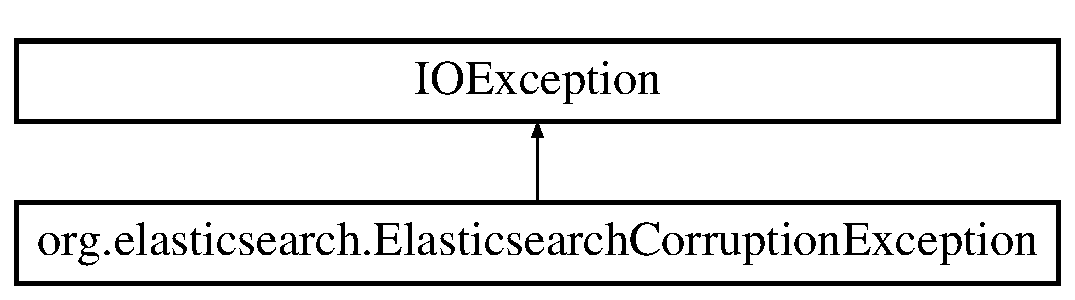
\includegraphics[height=2.000000cm]{classorg_1_1elasticsearch_1_1_elasticsearch_corruption_exception}
\end{center}
\end{figure}
\subsection*{Public Member Functions}
\begin{DoxyCompactItemize}
\item 
\hyperlink{classorg_1_1elasticsearch_1_1_elasticsearch_corruption_exception_adb85a4eb1872ef05cbbe11f6d193d91b}{Elasticsearch\+Corruption\+Exception} (String message)
\item 
\hyperlink{classorg_1_1elasticsearch_1_1_elasticsearch_corruption_exception_ab056deb66e8505b3b4d67e837af7c5bf}{Elasticsearch\+Corruption\+Exception} (Throwable ex)
\end{DoxyCompactItemize}


\subsection{Detailed Description}
This exception is thrown when Elasticsearch detects an inconsistency in one of it\textquotesingle{}s persistent files. 

\subsection{Constructor \& Destructor Documentation}
\hypertarget{classorg_1_1elasticsearch_1_1_elasticsearch_corruption_exception_adb85a4eb1872ef05cbbe11f6d193d91b}{}\label{classorg_1_1elasticsearch_1_1_elasticsearch_corruption_exception_adb85a4eb1872ef05cbbe11f6d193d91b} 
\index{org\+::elasticsearch\+::\+Elasticsearch\+Corruption\+Exception@{org\+::elasticsearch\+::\+Elasticsearch\+Corruption\+Exception}!Elasticsearch\+Corruption\+Exception@{Elasticsearch\+Corruption\+Exception}}
\index{Elasticsearch\+Corruption\+Exception@{Elasticsearch\+Corruption\+Exception}!org\+::elasticsearch\+::\+Elasticsearch\+Corruption\+Exception@{org\+::elasticsearch\+::\+Elasticsearch\+Corruption\+Exception}}
\subsubsection{\texorpdfstring{Elasticsearch\+Corruption\+Exception()}{ElasticsearchCorruptionException()}\hspace{0.1cm}{\footnotesize\ttfamily [1/2]}}
{\footnotesize\ttfamily org.\+elasticsearch.\+Elasticsearch\+Corruption\+Exception.\+Elasticsearch\+Corruption\+Exception (\begin{DoxyParamCaption}\item[{String}]{message }\end{DoxyParamCaption})}

Creates a new \hyperlink{classorg_1_1elasticsearch_1_1_elasticsearch_corruption_exception}{Elasticsearch\+Corruption\+Exception} 
\begin{DoxyParams}{Parameters}
{\em message} & the exception message. \\
\hline
\end{DoxyParams}
\hypertarget{classorg_1_1elasticsearch_1_1_elasticsearch_corruption_exception_ab056deb66e8505b3b4d67e837af7c5bf}{}\label{classorg_1_1elasticsearch_1_1_elasticsearch_corruption_exception_ab056deb66e8505b3b4d67e837af7c5bf} 
\index{org\+::elasticsearch\+::\+Elasticsearch\+Corruption\+Exception@{org\+::elasticsearch\+::\+Elasticsearch\+Corruption\+Exception}!Elasticsearch\+Corruption\+Exception@{Elasticsearch\+Corruption\+Exception}}
\index{Elasticsearch\+Corruption\+Exception@{Elasticsearch\+Corruption\+Exception}!org\+::elasticsearch\+::\+Elasticsearch\+Corruption\+Exception@{org\+::elasticsearch\+::\+Elasticsearch\+Corruption\+Exception}}
\subsubsection{\texorpdfstring{Elasticsearch\+Corruption\+Exception()}{ElasticsearchCorruptionException()}\hspace{0.1cm}{\footnotesize\ttfamily [2/2]}}
{\footnotesize\ttfamily org.\+elasticsearch.\+Elasticsearch\+Corruption\+Exception.\+Elasticsearch\+Corruption\+Exception (\begin{DoxyParamCaption}\item[{Throwable}]{ex }\end{DoxyParamCaption})}

Creates a new \hyperlink{classorg_1_1elasticsearch_1_1_elasticsearch_corruption_exception}{Elasticsearch\+Corruption\+Exception} with the given exceptions stacktrace. This constructor copies the stacktrace as well as the message from the given 
\begin{DoxyCode}
Throwable 
\end{DoxyCode}
 into this exception.


\begin{DoxyParams}{Parameters}
{\em ex} & the exception cause \\
\hline
\end{DoxyParams}


The documentation for this class was generated from the following file\+:\begin{DoxyCompactItemize}
\item 
core/src/main/java/org/elasticsearch/Elasticsearch\+Corruption\+Exception.\+java\end{DoxyCompactItemize}

\hypertarget{classorg_1_1elasticsearch_1_1_elasticsearch_exception}{}\section{org.\+elasticsearch.\+Elasticsearch\+Exception Class Reference}
\label{classorg_1_1elasticsearch_1_1_elasticsearch_exception}\index{org.\+elasticsearch.\+Elasticsearch\+Exception@{org.\+elasticsearch.\+Elasticsearch\+Exception}}
Inheritance diagram for org.\+elasticsearch.\+Elasticsearch\+Exception\+:\begin{figure}[H]
\begin{center}
\leavevmode
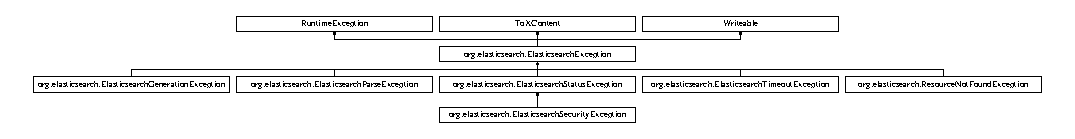
\includegraphics[height=1.422222cm]{classorg_1_1elasticsearch_1_1_elasticsearch_exception}
\end{center}
\end{figure}
\subsection*{Classes}
\begin{DoxyCompactItemize}
\item 
enum {\bfseries Elasticsearch\+Exception\+Handle}
\item 
interface {\bfseries Function\+That\+Throws\+I\+O\+Exception}
\end{DoxyCompactItemize}
\subsection*{Public Member Functions}
\begin{DoxyCompactItemize}
\item 
\hyperlink{classorg_1_1elasticsearch_1_1_elasticsearch_exception_ae6a6289693dfd265ad9167eb30918c3f}{Elasticsearch\+Exception} (Throwable cause)
\item 
\hyperlink{classorg_1_1elasticsearch_1_1_elasticsearch_exception_ae9bdc2247b5d219e66764dcf8ef4e7c6}{Elasticsearch\+Exception} (String msg, Object... args)
\item 
\hyperlink{classorg_1_1elasticsearch_1_1_elasticsearch_exception_a2202d9407b99327ee6af4af27d92f913}{Elasticsearch\+Exception} (String msg, Throwable cause, Object... args)
\item 
\hypertarget{classorg_1_1elasticsearch_1_1_elasticsearch_exception_a3c2822e315258b450247dc5f498a9638}{}\label{classorg_1_1elasticsearch_1_1_elasticsearch_exception_a3c2822e315258b450247dc5f498a9638} 
{\bfseries Elasticsearch\+Exception} (Stream\+Input in)  throws I\+O\+Exception 
\item 
void \hyperlink{classorg_1_1elasticsearch_1_1_elasticsearch_exception_a5810e3d73a8f132c0967e6a57732bc23}{add\+Header} (String key, String... value)
\item 
void \hyperlink{classorg_1_1elasticsearch_1_1_elasticsearch_exception_a2af671e59ace44acbfd37047341072ee}{add\+Header} (String key, List$<$ String $>$ value)
\item 
Set$<$ String $>$ \hyperlink{classorg_1_1elasticsearch_1_1_elasticsearch_exception_ac6b0fc84271df098d018e69db92058a4}{get\+Header\+Keys} ()
\item 
List$<$ String $>$ \hyperlink{classorg_1_1elasticsearch_1_1_elasticsearch_exception_ac5c7fe2597ce0b363d433503b23a1181}{get\+Header} (String key)
\item 
Rest\+Status \hyperlink{classorg_1_1elasticsearch_1_1_elasticsearch_exception_ad9c404eb416b323496900d737183875e}{status} ()
\item 
Throwable \hyperlink{classorg_1_1elasticsearch_1_1_elasticsearch_exception_afc4c4c4644fddfd06805fa19e65459fc}{unwrap\+Cause} ()
\item 
String \hyperlink{classorg_1_1elasticsearch_1_1_elasticsearch_exception_a4c3811c41b21d6c6dc7d7f5d97042e95}{get\+Detailed\+Message} ()
\item 
Throwable \hyperlink{classorg_1_1elasticsearch_1_1_elasticsearch_exception_a1d174a2312e18c883196ec07c87c2f50}{get\+Root\+Cause} ()
\item 
\hypertarget{classorg_1_1elasticsearch_1_1_elasticsearch_exception_a986086b6af724b62a245025a3f61a598}{}\label{classorg_1_1elasticsearch_1_1_elasticsearch_exception_a986086b6af724b62a245025a3f61a598} 
void {\bfseries write\+To} (Stream\+Output out)  throws I\+O\+Exception 
\item 
\hypertarget{classorg_1_1elasticsearch_1_1_elasticsearch_exception_a61f3e61b4485ddc1952fe4f3cf33fdee}{}\label{classorg_1_1elasticsearch_1_1_elasticsearch_exception_a61f3e61b4485ddc1952fe4f3cf33fdee} 
X\+Content\+Builder {\bfseries to\+X\+Content} (X\+Content\+Builder builder, Params params)  throws I\+O\+Exception 
\item 
\hyperlink{classorg_1_1elasticsearch_1_1_elasticsearch_exception}{Elasticsearch\+Exception} \mbox{[}$\,$\mbox{]} \hyperlink{classorg_1_1elasticsearch_1_1_elasticsearch_exception_aeda2312a330ae7c768410dafe13205e0}{guess\+Root\+Causes} ()
\item 
\hypertarget{classorg_1_1elasticsearch_1_1_elasticsearch_exception_a4eb4eeec440607f9c0bca7ec81016915}{}\label{classorg_1_1elasticsearch_1_1_elasticsearch_exception_a4eb4eeec440607f9c0bca7ec81016915} 
String {\bfseries to\+String} ()
\item 
\hypertarget{classorg_1_1elasticsearch_1_1_elasticsearch_exception_a7ff81e29624da75c45dfc9a26be82a4c}{}\label{classorg_1_1elasticsearch_1_1_elasticsearch_exception_a7ff81e29624da75c45dfc9a26be82a4c} 
Index {\bfseries get\+Index} ()
\item 
\hypertarget{classorg_1_1elasticsearch_1_1_elasticsearch_exception_ae9812bf2070dc9f33ecc37685e161f9b}{}\label{classorg_1_1elasticsearch_1_1_elasticsearch_exception_ae9812bf2070dc9f33ecc37685e161f9b} 
Shard\+Id {\bfseries get\+Shard\+Id} ()
\item 
\hypertarget{classorg_1_1elasticsearch_1_1_elasticsearch_exception_aba948242219b4ae9d3c03344706a5c9a}{}\label{classorg_1_1elasticsearch_1_1_elasticsearch_exception_aba948242219b4ae9d3c03344706a5c9a} 
void {\bfseries set\+Index} (Index index)
\item 
\hypertarget{classorg_1_1elasticsearch_1_1_elasticsearch_exception_a36dfe313effcd3f3347683ad108e48c5}{}\label{classorg_1_1elasticsearch_1_1_elasticsearch_exception_a36dfe313effcd3f3347683ad108e48c5} 
void {\bfseries set\+Index} (String index)
\item 
\hypertarget{classorg_1_1elasticsearch_1_1_elasticsearch_exception_abacd08f4449cc7f4fc07f63b52cb6897}{}\label{classorg_1_1elasticsearch_1_1_elasticsearch_exception_abacd08f4449cc7f4fc07f63b52cb6897} 
void {\bfseries set\+Shard} (Shard\+Id shard\+Id)
\item 
\hypertarget{classorg_1_1elasticsearch_1_1_elasticsearch_exception_a9dd84e12618a50990bc2eebd3ca0ecb7}{}\label{classorg_1_1elasticsearch_1_1_elasticsearch_exception_a9dd84e12618a50990bc2eebd3ca0ecb7} 
void {\bfseries set\+Shard} (String index, int shard\+Id)
\item 
\hypertarget{classorg_1_1elasticsearch_1_1_elasticsearch_exception_afbe0553fa9613d2390c7cc79f5e7828d}{}\label{classorg_1_1elasticsearch_1_1_elasticsearch_exception_afbe0553fa9613d2390c7cc79f5e7828d} 
void {\bfseries set\+Resources} (String type, String... id)
\item 
\hypertarget{classorg_1_1elasticsearch_1_1_elasticsearch_exception_af0d38f447e5c9f524525c3f591fb770f}{}\label{classorg_1_1elasticsearch_1_1_elasticsearch_exception_af0d38f447e5c9f524525c3f591fb770f} 
List$<$ String $>$ {\bfseries get\+Resource\+Id} ()
\item 
\hypertarget{classorg_1_1elasticsearch_1_1_elasticsearch_exception_a876aa049008d5bbc558ecafe77d246e6}{}\label{classorg_1_1elasticsearch_1_1_elasticsearch_exception_a876aa049008d5bbc558ecafe77d246e6} 
String {\bfseries get\+Resource\+Type} ()
\end{DoxyCompactItemize}
\subsection*{Static Public Member Functions}
\begin{DoxyCompactItemize}
\item 
\hypertarget{classorg_1_1elasticsearch_1_1_elasticsearch_exception_abfbb6b125f0ab0bcbb5f5bb080c2421c}{}\label{classorg_1_1elasticsearch_1_1_elasticsearch_exception_abfbb6b125f0ab0bcbb5f5bb080c2421c} 
static \hyperlink{classorg_1_1elasticsearch_1_1_elasticsearch_exception}{Elasticsearch\+Exception} {\bfseries read\+Exception} (Stream\+Input input, int id)  throws I\+O\+Exception 
\item 
static boolean \hyperlink{classorg_1_1elasticsearch_1_1_elasticsearch_exception_ab1d7b8b3886de9c733b6822408e118bf}{is\+Registered} (Class$<$? extends Throwable $>$ exception)
\item 
static int \hyperlink{classorg_1_1elasticsearch_1_1_elasticsearch_exception_aba2a26f7f9671d79bdd82f9c7de2bab7}{get\+Id} (Class$<$? extends \hyperlink{classorg_1_1elasticsearch_1_1_elasticsearch_exception}{Elasticsearch\+Exception} $>$ exception)
\item 
static void \hyperlink{classorg_1_1elasticsearch_1_1_elasticsearch_exception_a872e01b6335d7cffbe11ed3e6e9a4875}{to\+X\+Content} (X\+Content\+Builder builder, Params params, Throwable ex)  throws I\+O\+Exception 
\item 
static \hyperlink{classorg_1_1elasticsearch_1_1_elasticsearch_exception}{Elasticsearch\+Exception} \mbox{[}$\,$\mbox{]} \hyperlink{classorg_1_1elasticsearch_1_1_elasticsearch_exception_ad110e49bea5a310698f156fec22defcf}{guess\+Root\+Causes} (Throwable t)
\item 
static String \hyperlink{classorg_1_1elasticsearch_1_1_elasticsearch_exception_ac4f280f6f47ba5ba899ab0ec859253c3}{get\+Exception\+Name} (Throwable ex)
\item 
static$<$ T extends Throwable $>$ T \hyperlink{classorg_1_1elasticsearch_1_1_elasticsearch_exception_a5f0e567c795fbee6a3e7f475f0e88863}{read\+Stack\+Trace} (T throwable, Stream\+Input in)  throws I\+O\+Exception 
\item 
static$<$ T extends Throwable $>$ T \hyperlink{classorg_1_1elasticsearch_1_1_elasticsearch_exception_a22de3652428c7858c91a58c7d225a158}{write\+Stack\+Traces} (T throwable, Stream\+Output out)  throws I\+O\+Exception 
\item 
\hypertarget{classorg_1_1elasticsearch_1_1_elasticsearch_exception_ada161378a2ad7cd15936c42967e84274}{}\label{classorg_1_1elasticsearch_1_1_elasticsearch_exception_ada161378a2ad7cd15936c42967e84274} 
static void {\bfseries render\+Exception} (X\+Content\+Builder builder, Params params, Exception e)  throws I\+O\+Exception 
\end{DoxyCompactItemize}
\subsection*{Static Public Attributes}
\begin{DoxyCompactItemize}
\item 
\hypertarget{classorg_1_1elasticsearch_1_1_elasticsearch_exception_a7d8caafa358353c0522e6c06104fa0b7}{}\label{classorg_1_1elasticsearch_1_1_elasticsearch_exception_a7d8caafa358353c0522e6c06104fa0b7} 
static final String {\bfseries R\+E\+S\+T\+\_\+\+E\+X\+C\+E\+P\+T\+I\+O\+N\+\_\+\+S\+K\+I\+P\+\_\+\+C\+A\+U\+SE} = \char`\"{}rest.\+exception.\+cause.\+skip\char`\"{}
\item 
\hypertarget{classorg_1_1elasticsearch_1_1_elasticsearch_exception_a7306c9114fc2edbfb3075b2f199f2cca}{}\label{classorg_1_1elasticsearch_1_1_elasticsearch_exception_a7306c9114fc2edbfb3075b2f199f2cca} 
static final String {\bfseries R\+E\+S\+T\+\_\+\+E\+X\+C\+E\+P\+T\+I\+O\+N\+\_\+\+S\+K\+I\+P\+\_\+\+S\+T\+A\+C\+K\+\_\+\+T\+R\+A\+CE} = \char`\"{}rest.\+exception.\+stacktrace.\+skip\char`\"{}
\item 
\hypertarget{classorg_1_1elasticsearch_1_1_elasticsearch_exception_a9d080681e7c644310df9f46cbc109bd7}{}\label{classorg_1_1elasticsearch_1_1_elasticsearch_exception_a9d080681e7c644310df9f46cbc109bd7} 
static final boolean {\bfseries R\+E\+S\+T\+\_\+\+E\+X\+C\+E\+P\+T\+I\+O\+N\+\_\+\+S\+K\+I\+P\+\_\+\+S\+T\+A\+C\+K\+\_\+\+T\+R\+A\+C\+E\+\_\+\+D\+E\+F\+A\+U\+LT} = true
\item 
\hypertarget{classorg_1_1elasticsearch_1_1_elasticsearch_exception_ac4b24c901790fbef8a3fc1e7e63623d7}{}\label{classorg_1_1elasticsearch_1_1_elasticsearch_exception_ac4b24c901790fbef8a3fc1e7e63623d7} 
static final boolean {\bfseries R\+E\+S\+T\+\_\+\+E\+X\+C\+E\+P\+T\+I\+O\+N\+\_\+\+S\+K\+I\+P\+\_\+\+C\+A\+U\+S\+E\+\_\+\+D\+E\+F\+A\+U\+LT} = false
\end{DoxyCompactItemize}
\subsection*{Protected Member Functions}
\begin{DoxyCompactItemize}
\item 
void \hyperlink{classorg_1_1elasticsearch_1_1_elasticsearch_exception_a05b642f5d4bc79afdd5629c2a003c889}{inner\+To\+X\+Content} (X\+Content\+Builder builder, Params params)  throws I\+O\+Exception 
\item 
void \hyperlink{classorg_1_1elasticsearch_1_1_elasticsearch_exception_a0213b3882cf8a48f095b86df44951a96}{cause\+To\+X\+Content} (X\+Content\+Builder builder, Params params)  throws I\+O\+Exception 
\item 
\hypertarget{classorg_1_1elasticsearch_1_1_elasticsearch_exception_a016c38190f5f3c9cd6ea8ec564ddba82}{}\label{classorg_1_1elasticsearch_1_1_elasticsearch_exception_a016c38190f5f3c9cd6ea8ec564ddba82} 
final void {\bfseries render\+Header} (X\+Content\+Builder builder, Params params)  throws I\+O\+Exception 
\item 
\hypertarget{classorg_1_1elasticsearch_1_1_elasticsearch_exception_aa4623ee8db90b46459cfdadc1df14b80}{}\label{classorg_1_1elasticsearch_1_1_elasticsearch_exception_aa4623ee8db90b46459cfdadc1df14b80} 
String {\bfseries get\+Exception\+Name} ()
\end{DoxyCompactItemize}


\subsection{Detailed Description}
A base class for all elasticsearch exceptions. 

\subsection{Constructor \& Destructor Documentation}
\hypertarget{classorg_1_1elasticsearch_1_1_elasticsearch_exception_ae6a6289693dfd265ad9167eb30918c3f}{}\label{classorg_1_1elasticsearch_1_1_elasticsearch_exception_ae6a6289693dfd265ad9167eb30918c3f} 
\index{org\+::elasticsearch\+::\+Elasticsearch\+Exception@{org\+::elasticsearch\+::\+Elasticsearch\+Exception}!Elasticsearch\+Exception@{Elasticsearch\+Exception}}
\index{Elasticsearch\+Exception@{Elasticsearch\+Exception}!org\+::elasticsearch\+::\+Elasticsearch\+Exception@{org\+::elasticsearch\+::\+Elasticsearch\+Exception}}
\subsubsection{\texorpdfstring{Elasticsearch\+Exception()}{ElasticsearchException()}\hspace{0.1cm}{\footnotesize\ttfamily [1/3]}}
{\footnotesize\ttfamily org.\+elasticsearch.\+Elasticsearch\+Exception.\+Elasticsearch\+Exception (\begin{DoxyParamCaption}\item[{Throwable}]{cause }\end{DoxyParamCaption})}

Construct a {\ttfamily \hyperlink{classorg_1_1elasticsearch_1_1_elasticsearch_exception}{Elasticsearch\+Exception}} with the specified cause exception. \hypertarget{classorg_1_1elasticsearch_1_1_elasticsearch_exception_ae9bdc2247b5d219e66764dcf8ef4e7c6}{}\label{classorg_1_1elasticsearch_1_1_elasticsearch_exception_ae9bdc2247b5d219e66764dcf8ef4e7c6} 
\index{org\+::elasticsearch\+::\+Elasticsearch\+Exception@{org\+::elasticsearch\+::\+Elasticsearch\+Exception}!Elasticsearch\+Exception@{Elasticsearch\+Exception}}
\index{Elasticsearch\+Exception@{Elasticsearch\+Exception}!org\+::elasticsearch\+::\+Elasticsearch\+Exception@{org\+::elasticsearch\+::\+Elasticsearch\+Exception}}
\subsubsection{\texorpdfstring{Elasticsearch\+Exception()}{ElasticsearchException()}\hspace{0.1cm}{\footnotesize\ttfamily [2/3]}}
{\footnotesize\ttfamily org.\+elasticsearch.\+Elasticsearch\+Exception.\+Elasticsearch\+Exception (\begin{DoxyParamCaption}\item[{String}]{msg,  }\item[{Object...}]{args }\end{DoxyParamCaption})}

Construct a {\ttfamily \hyperlink{classorg_1_1elasticsearch_1_1_elasticsearch_exception}{Elasticsearch\+Exception}} with the specified detail message.

The message can be parameterized using {\ttfamily \{\}} as placeholders for the given arguments


\begin{DoxyParams}{Parameters}
{\em msg} & the detail message \\
\hline
{\em args} & the arguments for the message \\
\hline
\end{DoxyParams}
\hypertarget{classorg_1_1elasticsearch_1_1_elasticsearch_exception_a2202d9407b99327ee6af4af27d92f913}{}\label{classorg_1_1elasticsearch_1_1_elasticsearch_exception_a2202d9407b99327ee6af4af27d92f913} 
\index{org\+::elasticsearch\+::\+Elasticsearch\+Exception@{org\+::elasticsearch\+::\+Elasticsearch\+Exception}!Elasticsearch\+Exception@{Elasticsearch\+Exception}}
\index{Elasticsearch\+Exception@{Elasticsearch\+Exception}!org\+::elasticsearch\+::\+Elasticsearch\+Exception@{org\+::elasticsearch\+::\+Elasticsearch\+Exception}}
\subsubsection{\texorpdfstring{Elasticsearch\+Exception()}{ElasticsearchException()}\hspace{0.1cm}{\footnotesize\ttfamily [3/3]}}
{\footnotesize\ttfamily org.\+elasticsearch.\+Elasticsearch\+Exception.\+Elasticsearch\+Exception (\begin{DoxyParamCaption}\item[{String}]{msg,  }\item[{Throwable}]{cause,  }\item[{Object...}]{args }\end{DoxyParamCaption})}

Construct a {\ttfamily \hyperlink{classorg_1_1elasticsearch_1_1_elasticsearch_exception}{Elasticsearch\+Exception}} with the specified detail message and nested exception.

The message can be parameterized using {\ttfamily \{\}} as placeholders for the given arguments


\begin{DoxyParams}{Parameters}
{\em msg} & the detail message \\
\hline
{\em cause} & the nested exception \\
\hline
{\em args} & the arguments for the message \\
\hline
\end{DoxyParams}


\subsection{Member Function Documentation}
\hypertarget{classorg_1_1elasticsearch_1_1_elasticsearch_exception_a5810e3d73a8f132c0967e6a57732bc23}{}\label{classorg_1_1elasticsearch_1_1_elasticsearch_exception_a5810e3d73a8f132c0967e6a57732bc23} 
\index{org\+::elasticsearch\+::\+Elasticsearch\+Exception@{org\+::elasticsearch\+::\+Elasticsearch\+Exception}!add\+Header@{add\+Header}}
\index{add\+Header@{add\+Header}!org\+::elasticsearch\+::\+Elasticsearch\+Exception@{org\+::elasticsearch\+::\+Elasticsearch\+Exception}}
\subsubsection{\texorpdfstring{add\+Header()}{addHeader()}\hspace{0.1cm}{\footnotesize\ttfamily [1/2]}}
{\footnotesize\ttfamily void org.\+elasticsearch.\+Elasticsearch\+Exception.\+add\+Header (\begin{DoxyParamCaption}\item[{String}]{key,  }\item[{String...}]{value }\end{DoxyParamCaption})}

Adds a new header with the given key. This method will replace existing header if a header with the same key already exists \hypertarget{classorg_1_1elasticsearch_1_1_elasticsearch_exception_a2af671e59ace44acbfd37047341072ee}{}\label{classorg_1_1elasticsearch_1_1_elasticsearch_exception_a2af671e59ace44acbfd37047341072ee} 
\index{org\+::elasticsearch\+::\+Elasticsearch\+Exception@{org\+::elasticsearch\+::\+Elasticsearch\+Exception}!add\+Header@{add\+Header}}
\index{add\+Header@{add\+Header}!org\+::elasticsearch\+::\+Elasticsearch\+Exception@{org\+::elasticsearch\+::\+Elasticsearch\+Exception}}
\subsubsection{\texorpdfstring{add\+Header()}{addHeader()}\hspace{0.1cm}{\footnotesize\ttfamily [2/2]}}
{\footnotesize\ttfamily void org.\+elasticsearch.\+Elasticsearch\+Exception.\+add\+Header (\begin{DoxyParamCaption}\item[{String}]{key,  }\item[{List$<$ String $>$}]{value }\end{DoxyParamCaption})}

Adds a new header with the given key. This method will replace existing header if a header with the same key already exists \hypertarget{classorg_1_1elasticsearch_1_1_elasticsearch_exception_a0213b3882cf8a48f095b86df44951a96}{}\label{classorg_1_1elasticsearch_1_1_elasticsearch_exception_a0213b3882cf8a48f095b86df44951a96} 
\index{org\+::elasticsearch\+::\+Elasticsearch\+Exception@{org\+::elasticsearch\+::\+Elasticsearch\+Exception}!cause\+To\+X\+Content@{cause\+To\+X\+Content}}
\index{cause\+To\+X\+Content@{cause\+To\+X\+Content}!org\+::elasticsearch\+::\+Elasticsearch\+Exception@{org\+::elasticsearch\+::\+Elasticsearch\+Exception}}
\subsubsection{\texorpdfstring{cause\+To\+X\+Content()}{causeToXContent()}}
{\footnotesize\ttfamily void org.\+elasticsearch.\+Elasticsearch\+Exception.\+cause\+To\+X\+Content (\begin{DoxyParamCaption}\item[{X\+Content\+Builder}]{builder,  }\item[{Params}]{params }\end{DoxyParamCaption}) throws I\+O\+Exception\hspace{0.3cm}{\ttfamily [protected]}}

Renders a cause exception as xcontent \hypertarget{classorg_1_1elasticsearch_1_1_elasticsearch_exception_a4c3811c41b21d6c6dc7d7f5d97042e95}{}\label{classorg_1_1elasticsearch_1_1_elasticsearch_exception_a4c3811c41b21d6c6dc7d7f5d97042e95} 
\index{org\+::elasticsearch\+::\+Elasticsearch\+Exception@{org\+::elasticsearch\+::\+Elasticsearch\+Exception}!get\+Detailed\+Message@{get\+Detailed\+Message}}
\index{get\+Detailed\+Message@{get\+Detailed\+Message}!org\+::elasticsearch\+::\+Elasticsearch\+Exception@{org\+::elasticsearch\+::\+Elasticsearch\+Exception}}
\subsubsection{\texorpdfstring{get\+Detailed\+Message()}{getDetailedMessage()}}
{\footnotesize\ttfamily String org.\+elasticsearch.\+Elasticsearch\+Exception.\+get\+Detailed\+Message (\begin{DoxyParamCaption}{ }\end{DoxyParamCaption})}

Return the detail message, including the message from the nested exception if there is one. \hypertarget{classorg_1_1elasticsearch_1_1_elasticsearch_exception_ac4f280f6f47ba5ba899ab0ec859253c3}{}\label{classorg_1_1elasticsearch_1_1_elasticsearch_exception_ac4f280f6f47ba5ba899ab0ec859253c3} 
\index{org\+::elasticsearch\+::\+Elasticsearch\+Exception@{org\+::elasticsearch\+::\+Elasticsearch\+Exception}!get\+Exception\+Name@{get\+Exception\+Name}}
\index{get\+Exception\+Name@{get\+Exception\+Name}!org\+::elasticsearch\+::\+Elasticsearch\+Exception@{org\+::elasticsearch\+::\+Elasticsearch\+Exception}}
\subsubsection{\texorpdfstring{get\+Exception\+Name()}{getExceptionName()}}
{\footnotesize\ttfamily static String org.\+elasticsearch.\+Elasticsearch\+Exception.\+get\+Exception\+Name (\begin{DoxyParamCaption}\item[{Throwable}]{ex }\end{DoxyParamCaption})\hspace{0.3cm}{\ttfamily [static]}}

Returns a underscore case name for the given exception. This method strips {\ttfamily Elasticsearch} prefixes from exception names. \hypertarget{classorg_1_1elasticsearch_1_1_elasticsearch_exception_ac5c7fe2597ce0b363d433503b23a1181}{}\label{classorg_1_1elasticsearch_1_1_elasticsearch_exception_ac5c7fe2597ce0b363d433503b23a1181} 
\index{org\+::elasticsearch\+::\+Elasticsearch\+Exception@{org\+::elasticsearch\+::\+Elasticsearch\+Exception}!get\+Header@{get\+Header}}
\index{get\+Header@{get\+Header}!org\+::elasticsearch\+::\+Elasticsearch\+Exception@{org\+::elasticsearch\+::\+Elasticsearch\+Exception}}
\subsubsection{\texorpdfstring{get\+Header()}{getHeader()}}
{\footnotesize\ttfamily List$<$String$>$ org.\+elasticsearch.\+Elasticsearch\+Exception.\+get\+Header (\begin{DoxyParamCaption}\item[{String}]{key }\end{DoxyParamCaption})}

Returns the list of header values for the given key or
\begin{DoxyCode}
null 
\end{DoxyCode}
 if not header for the given key exists. \hypertarget{classorg_1_1elasticsearch_1_1_elasticsearch_exception_ac6b0fc84271df098d018e69db92058a4}{}\label{classorg_1_1elasticsearch_1_1_elasticsearch_exception_ac6b0fc84271df098d018e69db92058a4} 
\index{org\+::elasticsearch\+::\+Elasticsearch\+Exception@{org\+::elasticsearch\+::\+Elasticsearch\+Exception}!get\+Header\+Keys@{get\+Header\+Keys}}
\index{get\+Header\+Keys@{get\+Header\+Keys}!org\+::elasticsearch\+::\+Elasticsearch\+Exception@{org\+::elasticsearch\+::\+Elasticsearch\+Exception}}
\subsubsection{\texorpdfstring{get\+Header\+Keys()}{getHeaderKeys()}}
{\footnotesize\ttfamily Set$<$String$>$ org.\+elasticsearch.\+Elasticsearch\+Exception.\+get\+Header\+Keys (\begin{DoxyParamCaption}{ }\end{DoxyParamCaption})}

Returns a set of all header keys on this exception \hypertarget{classorg_1_1elasticsearch_1_1_elasticsearch_exception_aba2a26f7f9671d79bdd82f9c7de2bab7}{}\label{classorg_1_1elasticsearch_1_1_elasticsearch_exception_aba2a26f7f9671d79bdd82f9c7de2bab7} 
\index{org\+::elasticsearch\+::\+Elasticsearch\+Exception@{org\+::elasticsearch\+::\+Elasticsearch\+Exception}!get\+Id@{get\+Id}}
\index{get\+Id@{get\+Id}!org\+::elasticsearch\+::\+Elasticsearch\+Exception@{org\+::elasticsearch\+::\+Elasticsearch\+Exception}}
\subsubsection{\texorpdfstring{get\+Id()}{getId()}}
{\footnotesize\ttfamily static int org.\+elasticsearch.\+Elasticsearch\+Exception.\+get\+Id (\begin{DoxyParamCaption}\item[{Class$<$? extends \hyperlink{classorg_1_1elasticsearch_1_1_elasticsearch_exception}{Elasticsearch\+Exception} $>$}]{exception }\end{DoxyParamCaption})\hspace{0.3cm}{\ttfamily [static]}}

Returns the serialization id the given exception. \hypertarget{classorg_1_1elasticsearch_1_1_elasticsearch_exception_a1d174a2312e18c883196ec07c87c2f50}{}\label{classorg_1_1elasticsearch_1_1_elasticsearch_exception_a1d174a2312e18c883196ec07c87c2f50} 
\index{org\+::elasticsearch\+::\+Elasticsearch\+Exception@{org\+::elasticsearch\+::\+Elasticsearch\+Exception}!get\+Root\+Cause@{get\+Root\+Cause}}
\index{get\+Root\+Cause@{get\+Root\+Cause}!org\+::elasticsearch\+::\+Elasticsearch\+Exception@{org\+::elasticsearch\+::\+Elasticsearch\+Exception}}
\subsubsection{\texorpdfstring{get\+Root\+Cause()}{getRootCause()}}
{\footnotesize\ttfamily Throwable org.\+elasticsearch.\+Elasticsearch\+Exception.\+get\+Root\+Cause (\begin{DoxyParamCaption}{ }\end{DoxyParamCaption})}

Retrieve the innermost cause of this exception, if none, returns the current exception. \hypertarget{classorg_1_1elasticsearch_1_1_elasticsearch_exception_aeda2312a330ae7c768410dafe13205e0}{}\label{classorg_1_1elasticsearch_1_1_elasticsearch_exception_aeda2312a330ae7c768410dafe13205e0} 
\index{org\+::elasticsearch\+::\+Elasticsearch\+Exception@{org\+::elasticsearch\+::\+Elasticsearch\+Exception}!guess\+Root\+Causes@{guess\+Root\+Causes}}
\index{guess\+Root\+Causes@{guess\+Root\+Causes}!org\+::elasticsearch\+::\+Elasticsearch\+Exception@{org\+::elasticsearch\+::\+Elasticsearch\+Exception}}
\subsubsection{\texorpdfstring{guess\+Root\+Causes()}{guessRootCauses()}\hspace{0.1cm}{\footnotesize\ttfamily [1/2]}}
{\footnotesize\ttfamily \hyperlink{classorg_1_1elasticsearch_1_1_elasticsearch_exception}{Elasticsearch\+Exception} \mbox{[}$\,$\mbox{]} org.\+elasticsearch.\+Elasticsearch\+Exception.\+guess\+Root\+Causes (\begin{DoxyParamCaption}{ }\end{DoxyParamCaption})}

Returns the root cause of this exception or multiple if different shards caused different exceptions \hypertarget{classorg_1_1elasticsearch_1_1_elasticsearch_exception_ad110e49bea5a310698f156fec22defcf}{}\label{classorg_1_1elasticsearch_1_1_elasticsearch_exception_ad110e49bea5a310698f156fec22defcf} 
\index{org\+::elasticsearch\+::\+Elasticsearch\+Exception@{org\+::elasticsearch\+::\+Elasticsearch\+Exception}!guess\+Root\+Causes@{guess\+Root\+Causes}}
\index{guess\+Root\+Causes@{guess\+Root\+Causes}!org\+::elasticsearch\+::\+Elasticsearch\+Exception@{org\+::elasticsearch\+::\+Elasticsearch\+Exception}}
\subsubsection{\texorpdfstring{guess\+Root\+Causes()}{guessRootCauses()}\hspace{0.1cm}{\footnotesize\ttfamily [2/2]}}
{\footnotesize\ttfamily static \hyperlink{classorg_1_1elasticsearch_1_1_elasticsearch_exception}{Elasticsearch\+Exception} \mbox{[}$\,$\mbox{]} org.\+elasticsearch.\+Elasticsearch\+Exception.\+guess\+Root\+Causes (\begin{DoxyParamCaption}\item[{Throwable}]{t }\end{DoxyParamCaption})\hspace{0.3cm}{\ttfamily [static]}}

Returns the root cause of this exception or multiple if different shards caused different exceptions. If the given exception is not an instance of \hyperlink{}{org.\+elasticsearch.\+Elasticsearch\+Exception} an empty array is returned. \hypertarget{classorg_1_1elasticsearch_1_1_elasticsearch_exception_a05b642f5d4bc79afdd5629c2a003c889}{}\label{classorg_1_1elasticsearch_1_1_elasticsearch_exception_a05b642f5d4bc79afdd5629c2a003c889} 
\index{org\+::elasticsearch\+::\+Elasticsearch\+Exception@{org\+::elasticsearch\+::\+Elasticsearch\+Exception}!inner\+To\+X\+Content@{inner\+To\+X\+Content}}
\index{inner\+To\+X\+Content@{inner\+To\+X\+Content}!org\+::elasticsearch\+::\+Elasticsearch\+Exception@{org\+::elasticsearch\+::\+Elasticsearch\+Exception}}
\subsubsection{\texorpdfstring{inner\+To\+X\+Content()}{innerToXContent()}}
{\footnotesize\ttfamily void org.\+elasticsearch.\+Elasticsearch\+Exception.\+inner\+To\+X\+Content (\begin{DoxyParamCaption}\item[{X\+Content\+Builder}]{builder,  }\item[{Params}]{params }\end{DoxyParamCaption}) throws I\+O\+Exception\hspace{0.3cm}{\ttfamily [protected]}}

Renders additional per exception information into the xcontent \hypertarget{classorg_1_1elasticsearch_1_1_elasticsearch_exception_ab1d7b8b3886de9c733b6822408e118bf}{}\label{classorg_1_1elasticsearch_1_1_elasticsearch_exception_ab1d7b8b3886de9c733b6822408e118bf} 
\index{org\+::elasticsearch\+::\+Elasticsearch\+Exception@{org\+::elasticsearch\+::\+Elasticsearch\+Exception}!is\+Registered@{is\+Registered}}
\index{is\+Registered@{is\+Registered}!org\+::elasticsearch\+::\+Elasticsearch\+Exception@{org\+::elasticsearch\+::\+Elasticsearch\+Exception}}
\subsubsection{\texorpdfstring{is\+Registered()}{isRegistered()}}
{\footnotesize\ttfamily static boolean org.\+elasticsearch.\+Elasticsearch\+Exception.\+is\+Registered (\begin{DoxyParamCaption}\item[{Class$<$? extends Throwable $>$}]{exception }\end{DoxyParamCaption})\hspace{0.3cm}{\ttfamily [static]}}

Returns {\ttfamily true} iff the given class is a registered for an exception to be read. \hypertarget{classorg_1_1elasticsearch_1_1_elasticsearch_exception_a5f0e567c795fbee6a3e7f475f0e88863}{}\label{classorg_1_1elasticsearch_1_1_elasticsearch_exception_a5f0e567c795fbee6a3e7f475f0e88863} 
\index{org\+::elasticsearch\+::\+Elasticsearch\+Exception@{org\+::elasticsearch\+::\+Elasticsearch\+Exception}!read\+Stack\+Trace@{read\+Stack\+Trace}}
\index{read\+Stack\+Trace@{read\+Stack\+Trace}!org\+::elasticsearch\+::\+Elasticsearch\+Exception@{org\+::elasticsearch\+::\+Elasticsearch\+Exception}}
\subsubsection{\texorpdfstring{read\+Stack\+Trace()}{readStackTrace()}}
{\footnotesize\ttfamily static $<$T extends Throwable$>$ T org.\+elasticsearch.\+Elasticsearch\+Exception.\+read\+Stack\+Trace (\begin{DoxyParamCaption}\item[{T}]{throwable,  }\item[{Stream\+Input}]{in }\end{DoxyParamCaption}) throws I\+O\+Exception\hspace{0.3cm}{\ttfamily [static]}}

Deserializes stacktrace elements as well as suppressed exceptions from the given output stream and adds it to the given exception. \hypertarget{classorg_1_1elasticsearch_1_1_elasticsearch_exception_ad9c404eb416b323496900d737183875e}{}\label{classorg_1_1elasticsearch_1_1_elasticsearch_exception_ad9c404eb416b323496900d737183875e} 
\index{org\+::elasticsearch\+::\+Elasticsearch\+Exception@{org\+::elasticsearch\+::\+Elasticsearch\+Exception}!status@{status}}
\index{status@{status}!org\+::elasticsearch\+::\+Elasticsearch\+Exception@{org\+::elasticsearch\+::\+Elasticsearch\+Exception}}
\subsubsection{\texorpdfstring{status()}{status()}}
{\footnotesize\ttfamily Rest\+Status org.\+elasticsearch.\+Elasticsearch\+Exception.\+status (\begin{DoxyParamCaption}{ }\end{DoxyParamCaption})}

Returns the rest status code associated with this exception. \hypertarget{classorg_1_1elasticsearch_1_1_elasticsearch_exception_a872e01b6335d7cffbe11ed3e6e9a4875}{}\label{classorg_1_1elasticsearch_1_1_elasticsearch_exception_a872e01b6335d7cffbe11ed3e6e9a4875} 
\index{org\+::elasticsearch\+::\+Elasticsearch\+Exception@{org\+::elasticsearch\+::\+Elasticsearch\+Exception}!to\+X\+Content@{to\+X\+Content}}
\index{to\+X\+Content@{to\+X\+Content}!org\+::elasticsearch\+::\+Elasticsearch\+Exception@{org\+::elasticsearch\+::\+Elasticsearch\+Exception}}
\subsubsection{\texorpdfstring{to\+X\+Content()}{toXContent()}}
{\footnotesize\ttfamily static void org.\+elasticsearch.\+Elasticsearch\+Exception.\+to\+X\+Content (\begin{DoxyParamCaption}\item[{X\+Content\+Builder}]{builder,  }\item[{Params}]{params,  }\item[{Throwable}]{ex }\end{DoxyParamCaption}) throws I\+O\+Exception\hspace{0.3cm}{\ttfamily [static]}}

Statis to\+X\+Content helper method that also renders non \hyperlink{}{org.\+elasticsearch.\+Elasticsearch\+Exception} instances as X\+Content. \hypertarget{classorg_1_1elasticsearch_1_1_elasticsearch_exception_afc4c4c4644fddfd06805fa19e65459fc}{}\label{classorg_1_1elasticsearch_1_1_elasticsearch_exception_afc4c4c4644fddfd06805fa19e65459fc} 
\index{org\+::elasticsearch\+::\+Elasticsearch\+Exception@{org\+::elasticsearch\+::\+Elasticsearch\+Exception}!unwrap\+Cause@{unwrap\+Cause}}
\index{unwrap\+Cause@{unwrap\+Cause}!org\+::elasticsearch\+::\+Elasticsearch\+Exception@{org\+::elasticsearch\+::\+Elasticsearch\+Exception}}
\subsubsection{\texorpdfstring{unwrap\+Cause()}{unwrapCause()}}
{\footnotesize\ttfamily Throwable org.\+elasticsearch.\+Elasticsearch\+Exception.\+unwrap\+Cause (\begin{DoxyParamCaption}{ }\end{DoxyParamCaption})}

Unwraps the actual cause from the exception for cases when the exception is a \hyperlink{interfaceorg_1_1elasticsearch_1_1_elasticsearch_wrapper_exception}{Elasticsearch\+Wrapper\+Exception}.

\begin{DoxySeeAlso}{See also}
Exceptions\+Helper\+::unwrap\+Cause(\+Throwable) 
\end{DoxySeeAlso}
\hypertarget{classorg_1_1elasticsearch_1_1_elasticsearch_exception_a22de3652428c7858c91a58c7d225a158}{}\label{classorg_1_1elasticsearch_1_1_elasticsearch_exception_a22de3652428c7858c91a58c7d225a158} 
\index{org\+::elasticsearch\+::\+Elasticsearch\+Exception@{org\+::elasticsearch\+::\+Elasticsearch\+Exception}!write\+Stack\+Traces@{write\+Stack\+Traces}}
\index{write\+Stack\+Traces@{write\+Stack\+Traces}!org\+::elasticsearch\+::\+Elasticsearch\+Exception@{org\+::elasticsearch\+::\+Elasticsearch\+Exception}}
\subsubsection{\texorpdfstring{write\+Stack\+Traces()}{writeStackTraces()}}
{\footnotesize\ttfamily static $<$T extends Throwable$>$ T org.\+elasticsearch.\+Elasticsearch\+Exception.\+write\+Stack\+Traces (\begin{DoxyParamCaption}\item[{T}]{throwable,  }\item[{Stream\+Output}]{out }\end{DoxyParamCaption}) throws I\+O\+Exception\hspace{0.3cm}{\ttfamily [static]}}

Serializes the given exceptions stacktrace elements as well as it\textquotesingle{}s suppressed exceptions to the given output stream. 

The documentation for this class was generated from the following file\+:\begin{DoxyCompactItemize}
\item 
core/src/main/java/org/elasticsearch/Elasticsearch\+Exception.\+java\end{DoxyCompactItemize}

\hypertarget{classorg_1_1elasticsearch_1_1_elasticsearch_generation_exception}{}\section{org.\+elasticsearch.\+Elasticsearch\+Generation\+Exception Class Reference}
\label{classorg_1_1elasticsearch_1_1_elasticsearch_generation_exception}\index{org.\+elasticsearch.\+Elasticsearch\+Generation\+Exception@{org.\+elasticsearch.\+Elasticsearch\+Generation\+Exception}}
Inheritance diagram for org.\+elasticsearch.\+Elasticsearch\+Generation\+Exception\+:\begin{figure}[H]
\begin{center}
\leavevmode
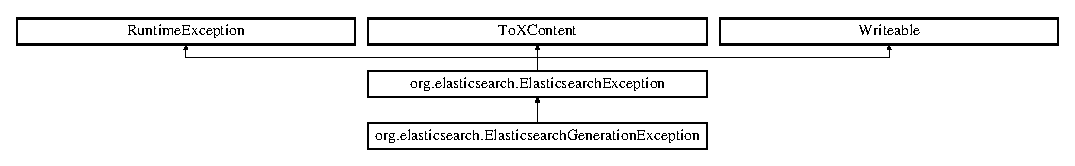
\includegraphics[height=1.777778cm]{classorg_1_1elasticsearch_1_1_elasticsearch_generation_exception}
\end{center}
\end{figure}
\subsection*{Public Member Functions}
\begin{DoxyCompactItemize}
\item 
\hypertarget{classorg_1_1elasticsearch_1_1_elasticsearch_generation_exception_a198115b04b0914bbabec38a9500ccc68}{}\label{classorg_1_1elasticsearch_1_1_elasticsearch_generation_exception_a198115b04b0914bbabec38a9500ccc68} 
{\bfseries Elasticsearch\+Generation\+Exception} (String msg)
\item 
\hypertarget{classorg_1_1elasticsearch_1_1_elasticsearch_generation_exception_a9caf798644d9ce43df2238af7a5b6bcb}{}\label{classorg_1_1elasticsearch_1_1_elasticsearch_generation_exception_a9caf798644d9ce43df2238af7a5b6bcb} 
{\bfseries Elasticsearch\+Generation\+Exception} (String msg, Throwable cause)
\item 
\hypertarget{classorg_1_1elasticsearch_1_1_elasticsearch_generation_exception_aeb911906c82f9f5f96348b7c747e6310}{}\label{classorg_1_1elasticsearch_1_1_elasticsearch_generation_exception_aeb911906c82f9f5f96348b7c747e6310} 
{\bfseries Elasticsearch\+Generation\+Exception} (Stream\+Input in)  throws I\+O\+Exception
\end{DoxyCompactItemize}
\subsection*{Additional Inherited Members}


\subsection{Detailed Description}
A generic exception indicating failure to generate. 

The documentation for this class was generated from the following file\+:\begin{DoxyCompactItemize}
\item 
core/src/main/java/org/elasticsearch/Elasticsearch\+Generation\+Exception.\+java\end{DoxyCompactItemize}

\hypertarget{classorg_1_1elasticsearch_1_1_elasticsearch_parse_exception}{}\section{org.\+elasticsearch.\+Elasticsearch\+Parse\+Exception Class Reference}
\label{classorg_1_1elasticsearch_1_1_elasticsearch_parse_exception}\index{org.\+elasticsearch.\+Elasticsearch\+Parse\+Exception@{org.\+elasticsearch.\+Elasticsearch\+Parse\+Exception}}
Inheritance diagram for org.\+elasticsearch.\+Elasticsearch\+Parse\+Exception\+:\begin{figure}[H]
\begin{center}
\leavevmode
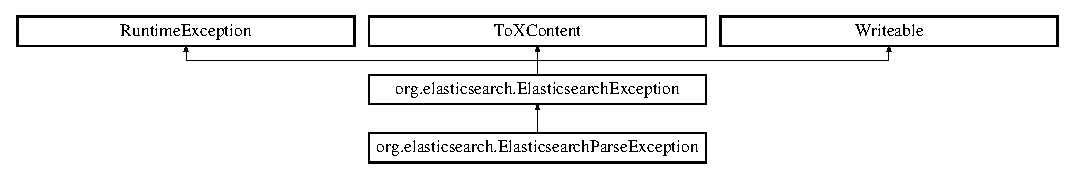
\includegraphics[height=1.958042cm]{classorg_1_1elasticsearch_1_1_elasticsearch_parse_exception}
\end{center}
\end{figure}
\subsection*{Public Member Functions}
\begin{DoxyCompactItemize}
\item 
\hypertarget{classorg_1_1elasticsearch_1_1_elasticsearch_parse_exception_ac90702099c505ee4b3df7b8bf6f1a3a7}{}\label{classorg_1_1elasticsearch_1_1_elasticsearch_parse_exception_ac90702099c505ee4b3df7b8bf6f1a3a7} 
{\bfseries Elasticsearch\+Parse\+Exception} (String msg, Object... args)
\item 
\hypertarget{classorg_1_1elasticsearch_1_1_elasticsearch_parse_exception_abe8a105a35b164de02a5300a44c22e59}{}\label{classorg_1_1elasticsearch_1_1_elasticsearch_parse_exception_abe8a105a35b164de02a5300a44c22e59} 
{\bfseries Elasticsearch\+Parse\+Exception} (String msg, Throwable cause, Object... args)
\item 
\hypertarget{classorg_1_1elasticsearch_1_1_elasticsearch_parse_exception_ae1d448d2e7ae564405df2e54e7de6cfb}{}\label{classorg_1_1elasticsearch_1_1_elasticsearch_parse_exception_ae1d448d2e7ae564405df2e54e7de6cfb} 
{\bfseries Elasticsearch\+Parse\+Exception} (Stream\+Input in)  throws I\+O\+Exception 
\item 
\hypertarget{classorg_1_1elasticsearch_1_1_elasticsearch_parse_exception_a7efb26db2918203591653f43fb55432d}{}\label{classorg_1_1elasticsearch_1_1_elasticsearch_parse_exception_a7efb26db2918203591653f43fb55432d} 
Rest\+Status {\bfseries status} ()
\end{DoxyCompactItemize}
\subsection*{Additional Inherited Members}


The documentation for this class was generated from the following file\+:\begin{DoxyCompactItemize}
\item 
core/src/main/java/org/elasticsearch/Elasticsearch\+Parse\+Exception.\+java\end{DoxyCompactItemize}

\hypertarget{classorg_1_1elasticsearch_1_1_elasticsearch_security_exception}{}\section{org.\+elasticsearch.\+Elasticsearch\+Security\+Exception Class Reference}
\label{classorg_1_1elasticsearch_1_1_elasticsearch_security_exception}\index{org.\+elasticsearch.\+Elasticsearch\+Security\+Exception@{org.\+elasticsearch.\+Elasticsearch\+Security\+Exception}}
Inheritance diagram for org.\+elasticsearch.\+Elasticsearch\+Security\+Exception\+:\begin{figure}[H]
\begin{center}
\leavevmode
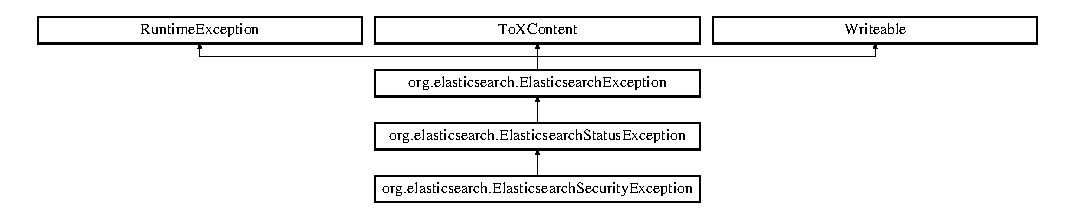
\includegraphics[height=2.488889cm]{classorg_1_1elasticsearch_1_1_elasticsearch_security_exception}
\end{center}
\end{figure}
\subsection*{Public Member Functions}
\begin{DoxyCompactItemize}
\item 
\hyperlink{classorg_1_1elasticsearch_1_1_elasticsearch_security_exception_a5f0e9afcfafaaaa5679204ae23c4d54d}{Elasticsearch\+Security\+Exception} (String msg, Rest\+Status status, Throwable cause, Object... args)
\item 
\hyperlink{classorg_1_1elasticsearch_1_1_elasticsearch_security_exception_aea6b2964cf3800b8213d147d5996f900}{Elasticsearch\+Security\+Exception} (String msg, Exception cause, Object... args)
\item 
\hyperlink{classorg_1_1elasticsearch_1_1_elasticsearch_security_exception_a88a789031337b5b83af8ae7a6e0d901f}{Elasticsearch\+Security\+Exception} (String msg, Object... args)
\item 
\hyperlink{classorg_1_1elasticsearch_1_1_elasticsearch_security_exception_a27d286caffe43a68193b8d71e7859e5a}{Elasticsearch\+Security\+Exception} (String msg, Rest\+Status status, Object... args)
\item 
\hyperlink{classorg_1_1elasticsearch_1_1_elasticsearch_security_exception_af0e61ba5f9f35c6f0d63b5b292d66712}{Elasticsearch\+Security\+Exception} (Stream\+Input in)  throws I\+O\+Exception 
\end{DoxyCompactItemize}
\subsection*{Additional Inherited Members}


\subsection{Detailed Description}
Generic security exception 

\subsection{Constructor \& Destructor Documentation}
\hypertarget{classorg_1_1elasticsearch_1_1_elasticsearch_security_exception_a5f0e9afcfafaaaa5679204ae23c4d54d}{}\label{classorg_1_1elasticsearch_1_1_elasticsearch_security_exception_a5f0e9afcfafaaaa5679204ae23c4d54d} 
\index{org\+::elasticsearch\+::\+Elasticsearch\+Security\+Exception@{org\+::elasticsearch\+::\+Elasticsearch\+Security\+Exception}!Elasticsearch\+Security\+Exception@{Elasticsearch\+Security\+Exception}}
\index{Elasticsearch\+Security\+Exception@{Elasticsearch\+Security\+Exception}!org\+::elasticsearch\+::\+Elasticsearch\+Security\+Exception@{org\+::elasticsearch\+::\+Elasticsearch\+Security\+Exception}}
\subsubsection{\texorpdfstring{Elasticsearch\+Security\+Exception()}{ElasticsearchSecurityException()}\hspace{0.1cm}{\footnotesize\ttfamily [1/5]}}
{\footnotesize\ttfamily org.\+elasticsearch.\+Elasticsearch\+Security\+Exception.\+Elasticsearch\+Security\+Exception (\begin{DoxyParamCaption}\item[{String}]{msg,  }\item[{Rest\+Status}]{status,  }\item[{Throwable}]{cause,  }\item[{Object...}]{args }\end{DoxyParamCaption})}

\hyperlink{classorg_1_1elasticsearch_1_1_build}{Build} the exception with a specific status and cause. \hypertarget{classorg_1_1elasticsearch_1_1_elasticsearch_security_exception_aea6b2964cf3800b8213d147d5996f900}{}\label{classorg_1_1elasticsearch_1_1_elasticsearch_security_exception_aea6b2964cf3800b8213d147d5996f900} 
\index{org\+::elasticsearch\+::\+Elasticsearch\+Security\+Exception@{org\+::elasticsearch\+::\+Elasticsearch\+Security\+Exception}!Elasticsearch\+Security\+Exception@{Elasticsearch\+Security\+Exception}}
\index{Elasticsearch\+Security\+Exception@{Elasticsearch\+Security\+Exception}!org\+::elasticsearch\+::\+Elasticsearch\+Security\+Exception@{org\+::elasticsearch\+::\+Elasticsearch\+Security\+Exception}}
\subsubsection{\texorpdfstring{Elasticsearch\+Security\+Exception()}{ElasticsearchSecurityException()}\hspace{0.1cm}{\footnotesize\ttfamily [2/5]}}
{\footnotesize\ttfamily org.\+elasticsearch.\+Elasticsearch\+Security\+Exception.\+Elasticsearch\+Security\+Exception (\begin{DoxyParamCaption}\item[{String}]{msg,  }\item[{Exception}]{cause,  }\item[{Object...}]{args }\end{DoxyParamCaption})}

\hyperlink{classorg_1_1elasticsearch_1_1_build}{Build} the exception with the status derived from the cause. \hypertarget{classorg_1_1elasticsearch_1_1_elasticsearch_security_exception_a88a789031337b5b83af8ae7a6e0d901f}{}\label{classorg_1_1elasticsearch_1_1_elasticsearch_security_exception_a88a789031337b5b83af8ae7a6e0d901f} 
\index{org\+::elasticsearch\+::\+Elasticsearch\+Security\+Exception@{org\+::elasticsearch\+::\+Elasticsearch\+Security\+Exception}!Elasticsearch\+Security\+Exception@{Elasticsearch\+Security\+Exception}}
\index{Elasticsearch\+Security\+Exception@{Elasticsearch\+Security\+Exception}!org\+::elasticsearch\+::\+Elasticsearch\+Security\+Exception@{org\+::elasticsearch\+::\+Elasticsearch\+Security\+Exception}}
\subsubsection{\texorpdfstring{Elasticsearch\+Security\+Exception()}{ElasticsearchSecurityException()}\hspace{0.1cm}{\footnotesize\ttfamily [3/5]}}
{\footnotesize\ttfamily org.\+elasticsearch.\+Elasticsearch\+Security\+Exception.\+Elasticsearch\+Security\+Exception (\begin{DoxyParamCaption}\item[{String}]{msg,  }\item[{Object...}]{args }\end{DoxyParamCaption})}

\hyperlink{classorg_1_1elasticsearch_1_1_build}{Build} the exception with a status of \hyperlink{}{Rest\+Status\#\+I\+N\+T\+E\+R\+N\+A\+L\+\_\+\+S\+E\+R\+V\+E\+R\+\_\+\+E\+R\+R\+OR} without a cause. \hypertarget{classorg_1_1elasticsearch_1_1_elasticsearch_security_exception_a27d286caffe43a68193b8d71e7859e5a}{}\label{classorg_1_1elasticsearch_1_1_elasticsearch_security_exception_a27d286caffe43a68193b8d71e7859e5a} 
\index{org\+::elasticsearch\+::\+Elasticsearch\+Security\+Exception@{org\+::elasticsearch\+::\+Elasticsearch\+Security\+Exception}!Elasticsearch\+Security\+Exception@{Elasticsearch\+Security\+Exception}}
\index{Elasticsearch\+Security\+Exception@{Elasticsearch\+Security\+Exception}!org\+::elasticsearch\+::\+Elasticsearch\+Security\+Exception@{org\+::elasticsearch\+::\+Elasticsearch\+Security\+Exception}}
\subsubsection{\texorpdfstring{Elasticsearch\+Security\+Exception()}{ElasticsearchSecurityException()}\hspace{0.1cm}{\footnotesize\ttfamily [4/5]}}
{\footnotesize\ttfamily org.\+elasticsearch.\+Elasticsearch\+Security\+Exception.\+Elasticsearch\+Security\+Exception (\begin{DoxyParamCaption}\item[{String}]{msg,  }\item[{Rest\+Status}]{status,  }\item[{Object...}]{args }\end{DoxyParamCaption})}

\hyperlink{classorg_1_1elasticsearch_1_1_build}{Build} the exception without a cause. \hypertarget{classorg_1_1elasticsearch_1_1_elasticsearch_security_exception_af0e61ba5f9f35c6f0d63b5b292d66712}{}\label{classorg_1_1elasticsearch_1_1_elasticsearch_security_exception_af0e61ba5f9f35c6f0d63b5b292d66712} 
\index{org\+::elasticsearch\+::\+Elasticsearch\+Security\+Exception@{org\+::elasticsearch\+::\+Elasticsearch\+Security\+Exception}!Elasticsearch\+Security\+Exception@{Elasticsearch\+Security\+Exception}}
\index{Elasticsearch\+Security\+Exception@{Elasticsearch\+Security\+Exception}!org\+::elasticsearch\+::\+Elasticsearch\+Security\+Exception@{org\+::elasticsearch\+::\+Elasticsearch\+Security\+Exception}}
\subsubsection{\texorpdfstring{Elasticsearch\+Security\+Exception()}{ElasticsearchSecurityException()}\hspace{0.1cm}{\footnotesize\ttfamily [5/5]}}
{\footnotesize\ttfamily org.\+elasticsearch.\+Elasticsearch\+Security\+Exception.\+Elasticsearch\+Security\+Exception (\begin{DoxyParamCaption}\item[{Stream\+Input}]{in }\end{DoxyParamCaption}) throws I\+O\+Exception}

Read from a stream. 

The documentation for this class was generated from the following file\+:\begin{DoxyCompactItemize}
\item 
core/src/main/java/org/elasticsearch/Elasticsearch\+Security\+Exception.\+java\end{DoxyCompactItemize}

\hypertarget{classorg_1_1elasticsearch_1_1_elasticsearch_status_exception}{}\section{org.\+elasticsearch.\+Elasticsearch\+Status\+Exception Class Reference}
\label{classorg_1_1elasticsearch_1_1_elasticsearch_status_exception}\index{org.\+elasticsearch.\+Elasticsearch\+Status\+Exception@{org.\+elasticsearch.\+Elasticsearch\+Status\+Exception}}
Inheritance diagram for org.\+elasticsearch.\+Elasticsearch\+Status\+Exception\+:\begin{figure}[H]
\begin{center}
\leavevmode
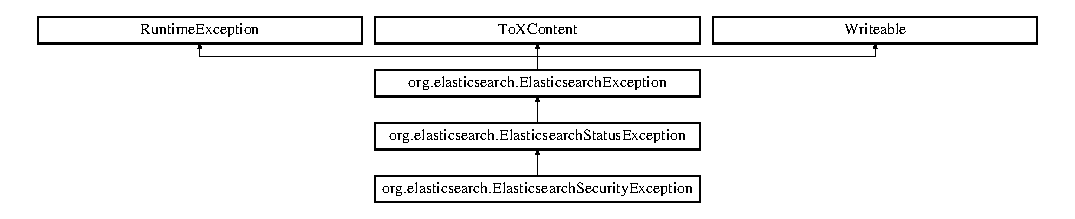
\includegraphics[height=2.488889cm]{classorg_1_1elasticsearch_1_1_elasticsearch_status_exception}
\end{center}
\end{figure}
\subsection*{Public Member Functions}
\begin{DoxyCompactItemize}
\item 
\hyperlink{classorg_1_1elasticsearch_1_1_elasticsearch_status_exception_a0e75cb4029aa054eb09e2fb524989c98}{Elasticsearch\+Status\+Exception} (String msg, Rest\+Status status, Throwable cause, Object... args)
\item 
\hyperlink{classorg_1_1elasticsearch_1_1_elasticsearch_status_exception_a8a059a544162d4a87a4808fc346e5f1e}{Elasticsearch\+Status\+Exception} (String msg, Rest\+Status status, Object... args)
\item 
\hyperlink{classorg_1_1elasticsearch_1_1_elasticsearch_status_exception_aea6fd693dc783d497b7ce62eb4804454}{Elasticsearch\+Status\+Exception} (Stream\+Input in)  throws I\+O\+Exception 
\item 
\hypertarget{classorg_1_1elasticsearch_1_1_elasticsearch_status_exception_a5ab3cb590573abd8fb8fe909a80b21e6}{}\label{classorg_1_1elasticsearch_1_1_elasticsearch_status_exception_a5ab3cb590573abd8fb8fe909a80b21e6} 
void {\bfseries write\+To} (Stream\+Output out)  throws I\+O\+Exception 
\item 
\hypertarget{classorg_1_1elasticsearch_1_1_elasticsearch_status_exception_aa86710084c254d7e78f10379b4de2d83}{}\label{classorg_1_1elasticsearch_1_1_elasticsearch_status_exception_aa86710084c254d7e78f10379b4de2d83} 
final Rest\+Status {\bfseries status} ()
\end{DoxyCompactItemize}
\subsection*{Additional Inherited Members}


\subsection{Detailed Description}
Exception who\textquotesingle{}s \hyperlink{}{Rest\+Status} is arbitrary rather than derived. Used, for example, by reindex-\/from-\/remote to wrap remote exceptions that contain a status. 

\subsection{Constructor \& Destructor Documentation}
\hypertarget{classorg_1_1elasticsearch_1_1_elasticsearch_status_exception_a0e75cb4029aa054eb09e2fb524989c98}{}\label{classorg_1_1elasticsearch_1_1_elasticsearch_status_exception_a0e75cb4029aa054eb09e2fb524989c98} 
\index{org\+::elasticsearch\+::\+Elasticsearch\+Status\+Exception@{org\+::elasticsearch\+::\+Elasticsearch\+Status\+Exception}!Elasticsearch\+Status\+Exception@{Elasticsearch\+Status\+Exception}}
\index{Elasticsearch\+Status\+Exception@{Elasticsearch\+Status\+Exception}!org\+::elasticsearch\+::\+Elasticsearch\+Status\+Exception@{org\+::elasticsearch\+::\+Elasticsearch\+Status\+Exception}}
\subsubsection{\texorpdfstring{Elasticsearch\+Status\+Exception()}{ElasticsearchStatusException()}\hspace{0.1cm}{\footnotesize\ttfamily [1/3]}}
{\footnotesize\ttfamily org.\+elasticsearch.\+Elasticsearch\+Status\+Exception.\+Elasticsearch\+Status\+Exception (\begin{DoxyParamCaption}\item[{String}]{msg,  }\item[{Rest\+Status}]{status,  }\item[{Throwable}]{cause,  }\item[{Object...}]{args }\end{DoxyParamCaption})}

\hyperlink{classorg_1_1elasticsearch_1_1_build}{Build} the exception with a specific status and cause. \hypertarget{classorg_1_1elasticsearch_1_1_elasticsearch_status_exception_a8a059a544162d4a87a4808fc346e5f1e}{}\label{classorg_1_1elasticsearch_1_1_elasticsearch_status_exception_a8a059a544162d4a87a4808fc346e5f1e} 
\index{org\+::elasticsearch\+::\+Elasticsearch\+Status\+Exception@{org\+::elasticsearch\+::\+Elasticsearch\+Status\+Exception}!Elasticsearch\+Status\+Exception@{Elasticsearch\+Status\+Exception}}
\index{Elasticsearch\+Status\+Exception@{Elasticsearch\+Status\+Exception}!org\+::elasticsearch\+::\+Elasticsearch\+Status\+Exception@{org\+::elasticsearch\+::\+Elasticsearch\+Status\+Exception}}
\subsubsection{\texorpdfstring{Elasticsearch\+Status\+Exception()}{ElasticsearchStatusException()}\hspace{0.1cm}{\footnotesize\ttfamily [2/3]}}
{\footnotesize\ttfamily org.\+elasticsearch.\+Elasticsearch\+Status\+Exception.\+Elasticsearch\+Status\+Exception (\begin{DoxyParamCaption}\item[{String}]{msg,  }\item[{Rest\+Status}]{status,  }\item[{Object...}]{args }\end{DoxyParamCaption})}

\hyperlink{classorg_1_1elasticsearch_1_1_build}{Build} the exception without a cause. \hypertarget{classorg_1_1elasticsearch_1_1_elasticsearch_status_exception_aea6fd693dc783d497b7ce62eb4804454}{}\label{classorg_1_1elasticsearch_1_1_elasticsearch_status_exception_aea6fd693dc783d497b7ce62eb4804454} 
\index{org\+::elasticsearch\+::\+Elasticsearch\+Status\+Exception@{org\+::elasticsearch\+::\+Elasticsearch\+Status\+Exception}!Elasticsearch\+Status\+Exception@{Elasticsearch\+Status\+Exception}}
\index{Elasticsearch\+Status\+Exception@{Elasticsearch\+Status\+Exception}!org\+::elasticsearch\+::\+Elasticsearch\+Status\+Exception@{org\+::elasticsearch\+::\+Elasticsearch\+Status\+Exception}}
\subsubsection{\texorpdfstring{Elasticsearch\+Status\+Exception()}{ElasticsearchStatusException()}\hspace{0.1cm}{\footnotesize\ttfamily [3/3]}}
{\footnotesize\ttfamily org.\+elasticsearch.\+Elasticsearch\+Status\+Exception.\+Elasticsearch\+Status\+Exception (\begin{DoxyParamCaption}\item[{Stream\+Input}]{in }\end{DoxyParamCaption}) throws I\+O\+Exception}

Read from a stream. 

The documentation for this class was generated from the following file\+:\begin{DoxyCompactItemize}
\item 
core/src/main/java/org/elasticsearch/Elasticsearch\+Status\+Exception.\+java\end{DoxyCompactItemize}

\hypertarget{classorg_1_1elasticsearch_1_1_elasticsearch_timeout_exception}{}\section{org.\+elasticsearch.\+Elasticsearch\+Timeout\+Exception Class Reference}
\label{classorg_1_1elasticsearch_1_1_elasticsearch_timeout_exception}\index{org.\+elasticsearch.\+Elasticsearch\+Timeout\+Exception@{org.\+elasticsearch.\+Elasticsearch\+Timeout\+Exception}}
Inheritance diagram for org.\+elasticsearch.\+Elasticsearch\+Timeout\+Exception\+:\begin{figure}[H]
\begin{center}
\leavevmode
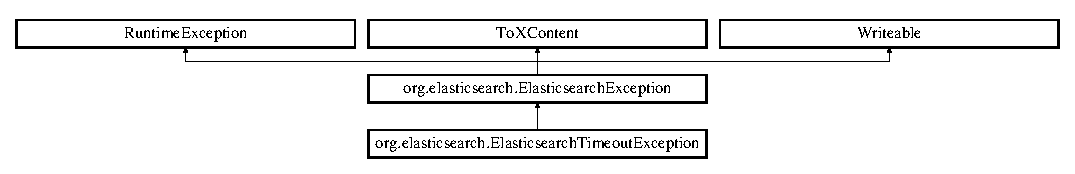
\includegraphics[height=1.891892cm]{classorg_1_1elasticsearch_1_1_elasticsearch_timeout_exception}
\end{center}
\end{figure}
\subsection*{Public Member Functions}
\begin{DoxyCompactItemize}
\item 
\hypertarget{classorg_1_1elasticsearch_1_1_elasticsearch_timeout_exception_a75e569df0ac602133309d78ac8531fce}{}\label{classorg_1_1elasticsearch_1_1_elasticsearch_timeout_exception_a75e569df0ac602133309d78ac8531fce} 
{\bfseries Elasticsearch\+Timeout\+Exception} (Stream\+Input in)  throws I\+O\+Exception 
\item 
\hypertarget{classorg_1_1elasticsearch_1_1_elasticsearch_timeout_exception_a31dd242c41e7ff8bf03820c2caeabf57}{}\label{classorg_1_1elasticsearch_1_1_elasticsearch_timeout_exception_a31dd242c41e7ff8bf03820c2caeabf57} 
{\bfseries Elasticsearch\+Timeout\+Exception} (Throwable cause)
\item 
\hypertarget{classorg_1_1elasticsearch_1_1_elasticsearch_timeout_exception_addec6eeeccdb9082d6beab843d5f6230}{}\label{classorg_1_1elasticsearch_1_1_elasticsearch_timeout_exception_addec6eeeccdb9082d6beab843d5f6230} 
{\bfseries Elasticsearch\+Timeout\+Exception} (String message, Object... args)
\item 
\hypertarget{classorg_1_1elasticsearch_1_1_elasticsearch_timeout_exception_adc4d4ca87a4c97153419994d176e1317}{}\label{classorg_1_1elasticsearch_1_1_elasticsearch_timeout_exception_adc4d4ca87a4c97153419994d176e1317} 
{\bfseries Elasticsearch\+Timeout\+Exception} (String message, Throwable cause, Object... args)
\end{DoxyCompactItemize}
\subsection*{Additional Inherited Members}


\subsection{Detailed Description}
The same as \hyperlink{}{java.\+util.\+concurrent.\+Timeout\+Exception} simply a runtime one. 

The documentation for this class was generated from the following file\+:\begin{DoxyCompactItemize}
\item 
core/src/main/java/org/elasticsearch/Elasticsearch\+Timeout\+Exception.\+java\end{DoxyCompactItemize}

\hypertarget{interfaceorg_1_1elasticsearch_1_1_elasticsearch_wrapper_exception}{}\section{org.\+elasticsearch.\+Elasticsearch\+Wrapper\+Exception Interface Reference}
\label{interfaceorg_1_1elasticsearch_1_1_elasticsearch_wrapper_exception}\index{org.\+elasticsearch.\+Elasticsearch\+Wrapper\+Exception@{org.\+elasticsearch.\+Elasticsearch\+Wrapper\+Exception}}
\subsection*{Public Member Functions}
\begin{DoxyCompactItemize}
\item 
\hypertarget{interfaceorg_1_1elasticsearch_1_1_elasticsearch_wrapper_exception_a5a693d40d1da0d4a2304b6c23591b18f}{}\label{interfaceorg_1_1elasticsearch_1_1_elasticsearch_wrapper_exception_a5a693d40d1da0d4a2304b6c23591b18f} 
Throwable {\bfseries get\+Cause} ()
\end{DoxyCompactItemize}


The documentation for this interface was generated from the following file\+:\begin{DoxyCompactItemize}
\item 
core/src/main/java/org/elasticsearch/Elasticsearch\+Wrapper\+Exception.\+java\end{DoxyCompactItemize}

\hypertarget{classorg_1_1elasticsearch_1_1_exceptions_helper}{}\section{org.\+elasticsearch.\+Exceptions\+Helper Class Reference}
\label{classorg_1_1elasticsearch_1_1_exceptions_helper}\index{org.\+elasticsearch.\+Exceptions\+Helper@{org.\+elasticsearch.\+Exceptions\+Helper}}
\subsection*{Classes}
\begin{DoxyCompactItemize}
\item 
class {\bfseries Group\+By}
\end{DoxyCompactItemize}
\subsection*{Static Public Member Functions}
\begin{DoxyCompactItemize}
\item 
\hypertarget{classorg_1_1elasticsearch_1_1_exceptions_helper_a58745605e2183728adcff0abba44738a}{}\label{classorg_1_1elasticsearch_1_1_exceptions_helper_a58745605e2183728adcff0abba44738a} 
static Runtime\+Exception {\bfseries convert\+To\+Runtime} (Exception e)
\item 
\hypertarget{classorg_1_1elasticsearch_1_1_exceptions_helper_a43f15321c7ff3620b362ababe8cf72c1}{}\label{classorg_1_1elasticsearch_1_1_exceptions_helper_a43f15321c7ff3620b362ababe8cf72c1} 
static \hyperlink{classorg_1_1elasticsearch_1_1_elasticsearch_exception}{Elasticsearch\+Exception} {\bfseries convert\+To\+Elastic} (Exception e)
\item 
\hypertarget{classorg_1_1elasticsearch_1_1_exceptions_helper_a867a606fb84e5669c66cd711e154ba01}{}\label{classorg_1_1elasticsearch_1_1_exceptions_helper_a867a606fb84e5669c66cd711e154ba01} 
static Rest\+Status {\bfseries status} (Throwable t)
\item 
\hypertarget{classorg_1_1elasticsearch_1_1_exceptions_helper_afe1e41350ff55d0a8c355fed092c8843}{}\label{classorg_1_1elasticsearch_1_1_exceptions_helper_afe1e41350ff55d0a8c355fed092c8843} 
static Throwable {\bfseries unwrap\+Cause} (Throwable t)
\item 
static String \hyperlink{classorg_1_1elasticsearch_1_1_exceptions_helper_a9ceadc9e3e73578bcf5ad6f14c91e6ff}{detailed\+Message} (Throwable t)
\item 
\hypertarget{classorg_1_1elasticsearch_1_1_exceptions_helper_a4b9859fad06d47581efc1449725e077c}{}\label{classorg_1_1elasticsearch_1_1_exceptions_helper_a4b9859fad06d47581efc1449725e077c} 
static String {\bfseries stack\+Trace} (Throwable e)
\item 
static$<$ T extends Throwable $>$ void \hyperlink{classorg_1_1elasticsearch_1_1_exceptions_helper_acf6601d79d7aaa8791ecc8847a480e4f}{rethrow\+And\+Suppress} (List$<$ T $>$ exceptions)  throws T 
\item 
static$<$ T extends Throwable $>$ void \hyperlink{classorg_1_1elasticsearch_1_1_exceptions_helper_ad3418e31f771224486cce3bb9c1992ff}{maybe\+Throw\+Runtime\+And\+Suppress} (List$<$ T $>$ exceptions)
\item 
\hypertarget{classorg_1_1elasticsearch_1_1_exceptions_helper_a621ce635df11ba76b4aea1685dcb31a1}{}\label{classorg_1_1elasticsearch_1_1_exceptions_helper_a621ce635df11ba76b4aea1685dcb31a1} 
static$<$ T extends Throwable $>$ T {\bfseries use\+Or\+Suppress} (T first, T second)
\item 
\hypertarget{classorg_1_1elasticsearch_1_1_exceptions_helper_a3dc53e2153ee007acf96a8099cbb49e7}{}\label{classorg_1_1elasticsearch_1_1_exceptions_helper_a3dc53e2153ee007acf96a8099cbb49e7} 
static I\+O\+Exception {\bfseries unwrap\+Corruption} (Throwable t)
\item 
\hypertarget{classorg_1_1elasticsearch_1_1_exceptions_helper_ab5b8cc274c7a8b3583a2bc4e70fecca5}{}\label{classorg_1_1elasticsearch_1_1_exceptions_helper_ab5b8cc274c7a8b3583a2bc4e70fecca5} 
static Throwable {\bfseries unwrap} (Throwable t, Class$<$?$>$... clazzes)
\item 
static boolean \hyperlink{classorg_1_1elasticsearch_1_1_exceptions_helper_adfbdc4265cf1618e246644191df6997d}{re\+Throw\+If\+Not\+Null} (@Nullable Throwable e)
\item 
static Shard\+Operation\+Failed\+Exception \mbox{[}$\,$\mbox{]} \hyperlink{classorg_1_1elasticsearch_1_1_exceptions_helper_aa969840c5155ff78386e8361b06e9307}{group\+By} (Shard\+Operation\+Failed\+Exception\mbox{[}$\,$\mbox{]} failures)
\end{DoxyCompactItemize}


\subsection{Member Function Documentation}
\hypertarget{classorg_1_1elasticsearch_1_1_exceptions_helper_a9ceadc9e3e73578bcf5ad6f14c91e6ff}{}\label{classorg_1_1elasticsearch_1_1_exceptions_helper_a9ceadc9e3e73578bcf5ad6f14c91e6ff} 
\index{org\+::elasticsearch\+::\+Exceptions\+Helper@{org\+::elasticsearch\+::\+Exceptions\+Helper}!detailed\+Message@{detailed\+Message}}
\index{detailed\+Message@{detailed\+Message}!org\+::elasticsearch\+::\+Exceptions\+Helper@{org\+::elasticsearch\+::\+Exceptions\+Helper}}
\subsubsection{\texorpdfstring{detailed\+Message()}{detailedMessage()}}
{\footnotesize\ttfamily static String org.\+elasticsearch.\+Exceptions\+Helper.\+detailed\+Message (\begin{DoxyParamCaption}\item[{Throwable}]{t }\end{DoxyParamCaption})\hspace{0.3cm}{\ttfamily [static]}}

\begin{DoxyRefDesc}{Deprecated}
\item[\hyperlink{deprecated__deprecated000001}{Deprecated}]Don\textquotesingle{}t swallow exceptions, allow them to propagate. \end{DoxyRefDesc}
\hypertarget{classorg_1_1elasticsearch_1_1_exceptions_helper_aa969840c5155ff78386e8361b06e9307}{}\label{classorg_1_1elasticsearch_1_1_exceptions_helper_aa969840c5155ff78386e8361b06e9307} 
\index{org\+::elasticsearch\+::\+Exceptions\+Helper@{org\+::elasticsearch\+::\+Exceptions\+Helper}!group\+By@{group\+By}}
\index{group\+By@{group\+By}!org\+::elasticsearch\+::\+Exceptions\+Helper@{org\+::elasticsearch\+::\+Exceptions\+Helper}}
\subsubsection{\texorpdfstring{group\+By()}{groupBy()}}
{\footnotesize\ttfamily static Shard\+Operation\+Failed\+Exception \mbox{[}$\,$\mbox{]} org.\+elasticsearch.\+Exceptions\+Helper.\+group\+By (\begin{DoxyParamCaption}\item[{Shard\+Operation\+Failed\+Exception \mbox{[}$\,$\mbox{]}}]{failures }\end{DoxyParamCaption})\hspace{0.3cm}{\ttfamily [static]}}

Deduplicate the failures by exception message and index. \hypertarget{classorg_1_1elasticsearch_1_1_exceptions_helper_ad3418e31f771224486cce3bb9c1992ff}{}\label{classorg_1_1elasticsearch_1_1_exceptions_helper_ad3418e31f771224486cce3bb9c1992ff} 
\index{org\+::elasticsearch\+::\+Exceptions\+Helper@{org\+::elasticsearch\+::\+Exceptions\+Helper}!maybe\+Throw\+Runtime\+And\+Suppress@{maybe\+Throw\+Runtime\+And\+Suppress}}
\index{maybe\+Throw\+Runtime\+And\+Suppress@{maybe\+Throw\+Runtime\+And\+Suppress}!org\+::elasticsearch\+::\+Exceptions\+Helper@{org\+::elasticsearch\+::\+Exceptions\+Helper}}
\subsubsection{\texorpdfstring{maybe\+Throw\+Runtime\+And\+Suppress()}{maybeThrowRuntimeAndSuppress()}}
{\footnotesize\ttfamily static $<$T extends Throwable$>$ void org.\+elasticsearch.\+Exceptions\+Helper.\+maybe\+Throw\+Runtime\+And\+Suppress (\begin{DoxyParamCaption}\item[{List$<$ T $>$}]{exceptions }\end{DoxyParamCaption})\hspace{0.3cm}{\ttfamily [static]}}

Throws a runtime exception with all given exceptions added as suppressed. If the given list is empty no exception is thrown \hypertarget{classorg_1_1elasticsearch_1_1_exceptions_helper_acf6601d79d7aaa8791ecc8847a480e4f}{}\label{classorg_1_1elasticsearch_1_1_exceptions_helper_acf6601d79d7aaa8791ecc8847a480e4f} 
\index{org\+::elasticsearch\+::\+Exceptions\+Helper@{org\+::elasticsearch\+::\+Exceptions\+Helper}!rethrow\+And\+Suppress@{rethrow\+And\+Suppress}}
\index{rethrow\+And\+Suppress@{rethrow\+And\+Suppress}!org\+::elasticsearch\+::\+Exceptions\+Helper@{org\+::elasticsearch\+::\+Exceptions\+Helper}}
\subsubsection{\texorpdfstring{rethrow\+And\+Suppress()}{rethrowAndSuppress()}}
{\footnotesize\ttfamily static $<$T extends Throwable$>$ void org.\+elasticsearch.\+Exceptions\+Helper.\+rethrow\+And\+Suppress (\begin{DoxyParamCaption}\item[{List$<$ T $>$}]{exceptions }\end{DoxyParamCaption}) throws T\hspace{0.3cm}{\ttfamily [static]}}

Rethrows the first exception in the list and adds all remaining to the suppressed list. If the given list is empty no exception is thrown \hypertarget{classorg_1_1elasticsearch_1_1_exceptions_helper_adfbdc4265cf1618e246644191df6997d}{}\label{classorg_1_1elasticsearch_1_1_exceptions_helper_adfbdc4265cf1618e246644191df6997d} 
\index{org\+::elasticsearch\+::\+Exceptions\+Helper@{org\+::elasticsearch\+::\+Exceptions\+Helper}!re\+Throw\+If\+Not\+Null@{re\+Throw\+If\+Not\+Null}}
\index{re\+Throw\+If\+Not\+Null@{re\+Throw\+If\+Not\+Null}!org\+::elasticsearch\+::\+Exceptions\+Helper@{org\+::elasticsearch\+::\+Exceptions\+Helper}}
\subsubsection{\texorpdfstring{re\+Throw\+If\+Not\+Null()}{reThrowIfNotNull()}}
{\footnotesize\ttfamily static boolean org.\+elasticsearch.\+Exceptions\+Helper.\+re\+Throw\+If\+Not\+Null (\begin{DoxyParamCaption}\item[{@Nullable Throwable}]{e }\end{DoxyParamCaption})\hspace{0.3cm}{\ttfamily [static]}}

Throws the specified exception. If null if specified then {\ttfamily true} is returned. 

The documentation for this class was generated from the following file\+:\begin{DoxyCompactItemize}
\item 
core/src/main/java/org/elasticsearch/Exceptions\+Helper.\+java\end{DoxyCompactItemize}

\hypertarget{classorg_1_1elasticsearch_1_1_resource_not_found_exception}{}\section{org.\+elasticsearch.\+Resource\+Not\+Found\+Exception Class Reference}
\label{classorg_1_1elasticsearch_1_1_resource_not_found_exception}\index{org.\+elasticsearch.\+Resource\+Not\+Found\+Exception@{org.\+elasticsearch.\+Resource\+Not\+Found\+Exception}}
Inheritance diagram for org.\+elasticsearch.\+Resource\+Not\+Found\+Exception\+:\begin{figure}[H]
\begin{center}
\leavevmode
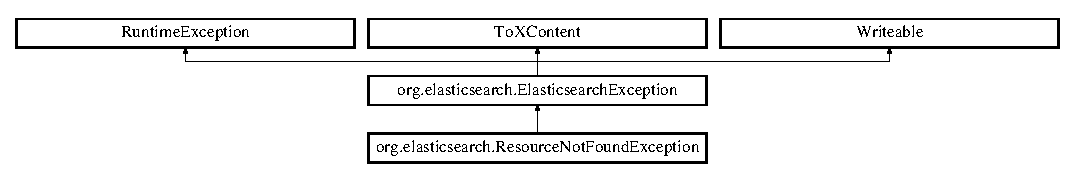
\includegraphics[height=1.958042cm]{classorg_1_1elasticsearch_1_1_resource_not_found_exception}
\end{center}
\end{figure}
\subsection*{Public Member Functions}
\begin{DoxyCompactItemize}
\item 
\hypertarget{classorg_1_1elasticsearch_1_1_resource_not_found_exception_aaa015c41f6418a1a9557dbfd1d5e74c9}{}\label{classorg_1_1elasticsearch_1_1_resource_not_found_exception_aaa015c41f6418a1a9557dbfd1d5e74c9} 
{\bfseries Resource\+Not\+Found\+Exception} (String msg, Object... args)
\item 
\hypertarget{classorg_1_1elasticsearch_1_1_resource_not_found_exception_ae6bda67ddb33d499b3b0e4f7c06bf008}{}\label{classorg_1_1elasticsearch_1_1_resource_not_found_exception_ae6bda67ddb33d499b3b0e4f7c06bf008} 
{\bfseries Resource\+Not\+Found\+Exception} (String msg, Throwable cause, Object... args)
\item 
\hypertarget{classorg_1_1elasticsearch_1_1_resource_not_found_exception_ab9a7c4ff2912fe0af5cab2030f47f63c}{}\label{classorg_1_1elasticsearch_1_1_resource_not_found_exception_ab9a7c4ff2912fe0af5cab2030f47f63c} 
{\bfseries Resource\+Not\+Found\+Exception} (Stream\+Input in)  throws I\+O\+Exception 
\item 
\hypertarget{classorg_1_1elasticsearch_1_1_resource_not_found_exception_aa65491eba4e2c10f1e9f5bd60a4dbf15}{}\label{classorg_1_1elasticsearch_1_1_resource_not_found_exception_aa65491eba4e2c10f1e9f5bd60a4dbf15} 
final Rest\+Status {\bfseries status} ()
\end{DoxyCompactItemize}
\subsection*{Additional Inherited Members}


\subsection{Detailed Description}
Generic \hyperlink{classorg_1_1elasticsearch_1_1_resource_not_found_exception}{Resource\+Not\+Found\+Exception} corresponding to the \hyperlink{}{Rest\+Status\#\+N\+O\+T\+\_\+\+F\+O\+U\+ND} status code 

The documentation for this class was generated from the following file\+:\begin{DoxyCompactItemize}
\item 
core/src/main/java/org/elasticsearch/Resource\+Not\+Found\+Exception.\+java\end{DoxyCompactItemize}

\hypertarget{classorg_1_1elasticsearch_1_1_special_permission}{}\section{org.\+elasticsearch.\+Special\+Permission Class Reference}
\label{classorg_1_1elasticsearch_1_1_special_permission}\index{org.\+elasticsearch.\+Special\+Permission@{org.\+elasticsearch.\+Special\+Permission}}
Inheritance diagram for org.\+elasticsearch.\+Special\+Permission\+:\begin{figure}[H]
\begin{center}
\leavevmode
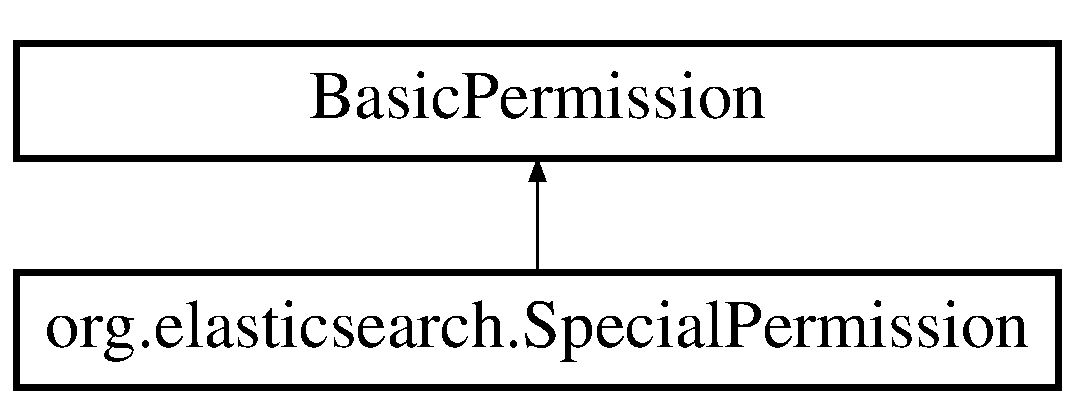
\includegraphics[height=2.000000cm]{classorg_1_1elasticsearch_1_1_special_permission}
\end{center}
\end{figure}
\subsection*{Public Member Functions}
\begin{DoxyCompactItemize}
\item 
\hyperlink{classorg_1_1elasticsearch_1_1_special_permission_ad7d44e1b12cf47115d5f4f0438238c82}{Special\+Permission} ()
\item 
\hyperlink{classorg_1_1elasticsearch_1_1_special_permission_abe8ca62b43aea4849338562577fc037b}{Special\+Permission} (String name, String actions)
\end{DoxyCompactItemize}


\subsection{Detailed Description}
Elasticsearch-\/specific permission to check before entering 
\begin{DoxyCode}
AccessController.doPrivileged() 
\end{DoxyCode}
 blocks. 

We try to avoid these blocks in our code and keep security simple, but we need them for a few special places to contain hacks for third party code, or dangerous things used by scripting engines. 

All normal code has this permission, but checking this before truncating the stack prevents unprivileged code (e.\+g. scripts), which do not have it, from gaining elevated privileges. 

In other words, don\textquotesingle{}t do this\+: ~\newline
 
\begin{DoxyPre}{\ttfamily 
  // throw away all information about caller and run with our own privs
  AccessController.doPrivileged(
   ...
  );
}\end{DoxyPre}
 ~\newline
 Instead do this; ~\newline
 
\begin{DoxyPre}{\ttfamily 
  // check caller first, to see if they should be allowed to do this
  SecurityManager sm = System.getSecurityManager();
  if (sm != null) \{
    sm.checkPermission(new SpecialPermission());
  \}
  // throw away all information about caller and run with our own privs
  AccessController.doPrivileged(
   ...
  );
}\end{DoxyPre}
 

\subsection{Constructor \& Destructor Documentation}
\hypertarget{classorg_1_1elasticsearch_1_1_special_permission_ad7d44e1b12cf47115d5f4f0438238c82}{}\label{classorg_1_1elasticsearch_1_1_special_permission_ad7d44e1b12cf47115d5f4f0438238c82} 
\index{org\+::elasticsearch\+::\+Special\+Permission@{org\+::elasticsearch\+::\+Special\+Permission}!Special\+Permission@{Special\+Permission}}
\index{Special\+Permission@{Special\+Permission}!org\+::elasticsearch\+::\+Special\+Permission@{org\+::elasticsearch\+::\+Special\+Permission}}
\subsubsection{\texorpdfstring{Special\+Permission()}{SpecialPermission()}\hspace{0.1cm}{\footnotesize\ttfamily [1/2]}}
{\footnotesize\ttfamily org.\+elasticsearch.\+Special\+Permission.\+Special\+Permission (\begin{DoxyParamCaption}{ }\end{DoxyParamCaption})}

Creates a new Special\+Permision object. \hypertarget{classorg_1_1elasticsearch_1_1_special_permission_abe8ca62b43aea4849338562577fc037b}{}\label{classorg_1_1elasticsearch_1_1_special_permission_abe8ca62b43aea4849338562577fc037b} 
\index{org\+::elasticsearch\+::\+Special\+Permission@{org\+::elasticsearch\+::\+Special\+Permission}!Special\+Permission@{Special\+Permission}}
\index{Special\+Permission@{Special\+Permission}!org\+::elasticsearch\+::\+Special\+Permission@{org\+::elasticsearch\+::\+Special\+Permission}}
\subsubsection{\texorpdfstring{Special\+Permission()}{SpecialPermission()}\hspace{0.1cm}{\footnotesize\ttfamily [2/2]}}
{\footnotesize\ttfamily org.\+elasticsearch.\+Special\+Permission.\+Special\+Permission (\begin{DoxyParamCaption}\item[{String}]{name,  }\item[{String}]{actions }\end{DoxyParamCaption})}

Creates a new \hyperlink{classorg_1_1elasticsearch_1_1_special_permission}{Special\+Permission} object. This constructor exists for use by the
\begin{DoxyCode}
Policy 
\end{DoxyCode}
 object to instantiate new Permission objects.


\begin{DoxyParams}{Parameters}
{\em name} & ignored \\
\hline
{\em actions} & ignored \\
\hline
\end{DoxyParams}


The documentation for this class was generated from the following file\+:\begin{DoxyCompactItemize}
\item 
core/src/main/java/org/elasticsearch/Special\+Permission.\+java\end{DoxyCompactItemize}

\hypertarget{classorg_1_1elasticsearch_1_1_version}{}\section{org.\+elasticsearch.\+Version Class Reference}
\label{classorg_1_1elasticsearch_1_1_version}\index{org.\+elasticsearch.\+Version@{org.\+elasticsearch.\+Version}}
\subsection*{Public Member Functions}
\begin{DoxyCompactItemize}
\item 
\hypertarget{classorg_1_1elasticsearch_1_1_version_a11d948e265c4257f9448d85eee90825c}{}\label{classorg_1_1elasticsearch_1_1_version_a11d948e265c4257f9448d85eee90825c} 
boolean {\bfseries after} (\hyperlink{classorg_1_1elasticsearch_1_1_version}{Version} version)
\item 
\hypertarget{classorg_1_1elasticsearch_1_1_version_ae710178d9a0c322226e5790df003e3c9}{}\label{classorg_1_1elasticsearch_1_1_version_ae710178d9a0c322226e5790df003e3c9} 
boolean {\bfseries on\+Or\+After} (\hyperlink{classorg_1_1elasticsearch_1_1_version}{Version} version)
\item 
\hypertarget{classorg_1_1elasticsearch_1_1_version_a49e0c223a8e06afcd81731643b3c4316}{}\label{classorg_1_1elasticsearch_1_1_version_a49e0c223a8e06afcd81731643b3c4316} 
boolean {\bfseries before} (\hyperlink{classorg_1_1elasticsearch_1_1_version}{Version} version)
\item 
\hypertarget{classorg_1_1elasticsearch_1_1_version_a9fbe54cd0de0cd556a7d1b4505965d0c}{}\label{classorg_1_1elasticsearch_1_1_version_a9fbe54cd0de0cd556a7d1b4505965d0c} 
boolean {\bfseries on\+Or\+Before} (\hyperlink{classorg_1_1elasticsearch_1_1_version}{Version} version)
\item 
\hyperlink{classorg_1_1elasticsearch_1_1_version}{Version} \hyperlink{classorg_1_1elasticsearch_1_1_version_af19fa9cd6c365d9b6f1ab0003463e259}{minimum\+Compatibility\+Version} ()
\item 
\hypertarget{classorg_1_1elasticsearch_1_1_version_add4796816f356001d35f37ce210fe0d7}{}\label{classorg_1_1elasticsearch_1_1_version_add4796816f356001d35f37ce210fe0d7} 
String {\bfseries to\+String} ()
\item 
\hypertarget{classorg_1_1elasticsearch_1_1_version_a1b419a92f27a4035da69fc93e5ad2bbd}{}\label{classorg_1_1elasticsearch_1_1_version_a1b419a92f27a4035da69fc93e5ad2bbd} 
boolean {\bfseries equals} (Object o)
\item 
\hypertarget{classorg_1_1elasticsearch_1_1_version_a6e5d8805ef643a4a5c5585181550a82c}{}\label{classorg_1_1elasticsearch_1_1_version_a6e5d8805ef643a4a5c5585181550a82c} 
int {\bfseries hash\+Code} ()
\item 
\hypertarget{classorg_1_1elasticsearch_1_1_version_af128cc4619c4cc2cc5112b0de7b6fe71}{}\label{classorg_1_1elasticsearch_1_1_version_af128cc4619c4cc2cc5112b0de7b6fe71} 
boolean {\bfseries is\+Beta} ()
\item 
boolean \hyperlink{classorg_1_1elasticsearch_1_1_version_a560e0d9bdd52a687b6920df72199dbec}{is\+Alpha} ()
\item 
\hypertarget{classorg_1_1elasticsearch_1_1_version_a2141338d4dbe770bc51ab06f41183afb}{}\label{classorg_1_1elasticsearch_1_1_version_a2141338d4dbe770bc51ab06f41183afb} 
boolean {\bfseries is\+RC} ()
\end{DoxyCompactItemize}
\subsection*{Static Public Member Functions}
\begin{DoxyCompactItemize}
\item 
\hypertarget{classorg_1_1elasticsearch_1_1_version_a5727ea8291db517bb5f34a1d260ae52b}{}\label{classorg_1_1elasticsearch_1_1_version_a5727ea8291db517bb5f34a1d260ae52b} 
static \hyperlink{classorg_1_1elasticsearch_1_1_version}{Version} {\bfseries read\+Version} (Stream\+Input in)  throws I\+O\+Exception 
\item 
\hypertarget{classorg_1_1elasticsearch_1_1_version_a50d41630cc6151425839dc725ff218e9}{}\label{classorg_1_1elasticsearch_1_1_version_a50d41630cc6151425839dc725ff218e9} 
static \hyperlink{classorg_1_1elasticsearch_1_1_version}{Version} {\bfseries from\+Id} (int id)
\item 
static \hyperlink{classorg_1_1elasticsearch_1_1_version}{Version} \hyperlink{classorg_1_1elasticsearch_1_1_version_a6c61e82b33e6a02aeea43e0d5db810df}{index\+Created} (Settings index\+Settings)
\item 
\hypertarget{classorg_1_1elasticsearch_1_1_version_aa3c90bc0dea3484e4b887ab6dc030972}{}\label{classorg_1_1elasticsearch_1_1_version_aa3c90bc0dea3484e4b887ab6dc030972} 
static void {\bfseries write\+Version} (\hyperlink{classorg_1_1elasticsearch_1_1_version}{Version} version, Stream\+Output out)  throws I\+O\+Exception 
\item 
static \hyperlink{classorg_1_1elasticsearch_1_1_version}{Version} \hyperlink{classorg_1_1elasticsearch_1_1_version_ab8ee3b9ccaaccbf4980b74541a5f7681}{smallest} (\hyperlink{classorg_1_1elasticsearch_1_1_version}{Version} version1, \hyperlink{classorg_1_1elasticsearch_1_1_version}{Version} version2)
\item 
static \hyperlink{classorg_1_1elasticsearch_1_1_version}{Version} \hyperlink{classorg_1_1elasticsearch_1_1_version_a86635d26e4db619bfa9f33cee16be1e5}{from\+String} (String version)
\item 
\hypertarget{classorg_1_1elasticsearch_1_1_version_a0e8c9543e498ded25a46579eef920a3d}{}\label{classorg_1_1elasticsearch_1_1_version_a0e8c9543e498ded25a46579eef920a3d} 
static void {\bfseries main} (String\mbox{[}$\,$\mbox{]} args)
\end{DoxyCompactItemize}
\subsection*{Public Attributes}
\begin{DoxyCompactItemize}
\item 
\hypertarget{classorg_1_1elasticsearch_1_1_version_a7d0441a885a0f1709edc88263f0be6ff}{}\label{classorg_1_1elasticsearch_1_1_version_a7d0441a885a0f1709edc88263f0be6ff} 
final int {\bfseries id}
\item 
\hypertarget{classorg_1_1elasticsearch_1_1_version_a31ea702852277aa45220b971ea4bf680}{}\label{classorg_1_1elasticsearch_1_1_version_a31ea702852277aa45220b971ea4bf680} 
final byte {\bfseries major}
\item 
\hypertarget{classorg_1_1elasticsearch_1_1_version_ae95e9b67f246cabaf72000b40ebad7ce}{}\label{classorg_1_1elasticsearch_1_1_version_ae95e9b67f246cabaf72000b40ebad7ce} 
final byte {\bfseries minor}
\item 
\hypertarget{classorg_1_1elasticsearch_1_1_version_acd9113301ce4c217150d91740b194242}{}\label{classorg_1_1elasticsearch_1_1_version_acd9113301ce4c217150d91740b194242} 
final byte {\bfseries revision}
\item 
\hypertarget{classorg_1_1elasticsearch_1_1_version_ae323f5d192871d0d18a36ff7f4c91b7d}{}\label{classorg_1_1elasticsearch_1_1_version_ae323f5d192871d0d18a36ff7f4c91b7d} 
final byte {\bfseries build}
\item 
\hypertarget{classorg_1_1elasticsearch_1_1_version_a040e34412520e347db6f3a4035a31833}{}\label{classorg_1_1elasticsearch_1_1_version_a040e34412520e347db6f3a4035a31833} 
final org.\+apache.\+lucene.\+util.\+Version {\bfseries lucene\+Version}
\end{DoxyCompactItemize}
\subsection*{Static Public Attributes}
\begin{DoxyCompactItemize}
\item 
\hypertarget{classorg_1_1elasticsearch_1_1_version_ae67971c05a341e8421ee39d8e77d508d}{}\label{classorg_1_1elasticsearch_1_1_version_ae67971c05a341e8421ee39d8e77d508d} 
static final int {\bfseries V\+\_\+2\+\_\+0\+\_\+0\+\_\+beta1\+\_\+\+ID} = 2000001
\item 
\hypertarget{classorg_1_1elasticsearch_1_1_version_a4b79c3ca4e491ec29822ca019e695a02}{}\label{classorg_1_1elasticsearch_1_1_version_a4b79c3ca4e491ec29822ca019e695a02} 
static final \hyperlink{classorg_1_1elasticsearch_1_1_version}{Version} {\bfseries V\+\_\+2\+\_\+0\+\_\+0\+\_\+beta1} = new \hyperlink{classorg_1_1elasticsearch_1_1_version}{Version}(V\+\_\+2\+\_\+0\+\_\+0\+\_\+beta1\+\_\+\+ID, org.\+apache.\+lucene.\+util.\+Version.\+L\+U\+C\+E\+N\+E\+\_\+5\+\_\+2\+\_\+1)
\item 
\hypertarget{classorg_1_1elasticsearch_1_1_version_a510d159b11776327ae3867239aec1146}{}\label{classorg_1_1elasticsearch_1_1_version_a510d159b11776327ae3867239aec1146} 
static final int {\bfseries V\+\_\+2\+\_\+0\+\_\+0\+\_\+beta2\+\_\+\+ID} = 2000002
\item 
\hypertarget{classorg_1_1elasticsearch_1_1_version_a21a68fea86cce98773377c6e65156507}{}\label{classorg_1_1elasticsearch_1_1_version_a21a68fea86cce98773377c6e65156507} 
static final \hyperlink{classorg_1_1elasticsearch_1_1_version}{Version} {\bfseries V\+\_\+2\+\_\+0\+\_\+0\+\_\+beta2} = new \hyperlink{classorg_1_1elasticsearch_1_1_version}{Version}(V\+\_\+2\+\_\+0\+\_\+0\+\_\+beta2\+\_\+\+ID, org.\+apache.\+lucene.\+util.\+Version.\+L\+U\+C\+E\+N\+E\+\_\+5\+\_\+2\+\_\+1)
\item 
\hypertarget{classorg_1_1elasticsearch_1_1_version_a697af71ea3287723d904b1f69726debf}{}\label{classorg_1_1elasticsearch_1_1_version_a697af71ea3287723d904b1f69726debf} 
static final int {\bfseries V\+\_\+2\+\_\+0\+\_\+0\+\_\+rc1\+\_\+\+ID} = 2000051
\item 
\hypertarget{classorg_1_1elasticsearch_1_1_version_a897706a30581a547efec56f4b4c4d03a}{}\label{classorg_1_1elasticsearch_1_1_version_a897706a30581a547efec56f4b4c4d03a} 
static final \hyperlink{classorg_1_1elasticsearch_1_1_version}{Version} {\bfseries V\+\_\+2\+\_\+0\+\_\+0\+\_\+rc1} = new \hyperlink{classorg_1_1elasticsearch_1_1_version}{Version}(V\+\_\+2\+\_\+0\+\_\+0\+\_\+rc1\+\_\+\+ID, org.\+apache.\+lucene.\+util.\+Version.\+L\+U\+C\+E\+N\+E\+\_\+5\+\_\+2\+\_\+1)
\item 
\hypertarget{classorg_1_1elasticsearch_1_1_version_a06e13e33c869f67483ce8458d78b5bf7}{}\label{classorg_1_1elasticsearch_1_1_version_a06e13e33c869f67483ce8458d78b5bf7} 
static final int {\bfseries V\+\_\+2\+\_\+0\+\_\+0\+\_\+\+ID} = 2000099
\item 
\hypertarget{classorg_1_1elasticsearch_1_1_version_a87b611e0ba88f06806b8edf8a381bda2}{}\label{classorg_1_1elasticsearch_1_1_version_a87b611e0ba88f06806b8edf8a381bda2} 
static final \hyperlink{classorg_1_1elasticsearch_1_1_version}{Version} {\bfseries V\+\_\+2\+\_\+0\+\_\+0} = new \hyperlink{classorg_1_1elasticsearch_1_1_version}{Version}(V\+\_\+2\+\_\+0\+\_\+0\+\_\+\+ID, org.\+apache.\+lucene.\+util.\+Version.\+L\+U\+C\+E\+N\+E\+\_\+5\+\_\+2\+\_\+1)
\item 
\hypertarget{classorg_1_1elasticsearch_1_1_version_a3eee27028c8f1d3a9d7d84ccf73932da}{}\label{classorg_1_1elasticsearch_1_1_version_a3eee27028c8f1d3a9d7d84ccf73932da} 
static final int {\bfseries V\+\_\+2\+\_\+0\+\_\+1\+\_\+\+ID} = 2000199
\item 
\hypertarget{classorg_1_1elasticsearch_1_1_version_a68b3bf2ba758c57455783749a491c38a}{}\label{classorg_1_1elasticsearch_1_1_version_a68b3bf2ba758c57455783749a491c38a} 
static final \hyperlink{classorg_1_1elasticsearch_1_1_version}{Version} {\bfseries V\+\_\+2\+\_\+0\+\_\+1} = new \hyperlink{classorg_1_1elasticsearch_1_1_version}{Version}(V\+\_\+2\+\_\+0\+\_\+1\+\_\+\+ID, org.\+apache.\+lucene.\+util.\+Version.\+L\+U\+C\+E\+N\+E\+\_\+5\+\_\+2\+\_\+1)
\item 
\hypertarget{classorg_1_1elasticsearch_1_1_version_a3860ab6ac12eb0aef3e2c710e3de2b8e}{}\label{classorg_1_1elasticsearch_1_1_version_a3860ab6ac12eb0aef3e2c710e3de2b8e} 
static final int {\bfseries V\+\_\+2\+\_\+0\+\_\+2\+\_\+\+ID} = 2000299
\item 
\hypertarget{classorg_1_1elasticsearch_1_1_version_a48a99fae1a819d275c3683f762a0a984}{}\label{classorg_1_1elasticsearch_1_1_version_a48a99fae1a819d275c3683f762a0a984} 
static final \hyperlink{classorg_1_1elasticsearch_1_1_version}{Version} {\bfseries V\+\_\+2\+\_\+0\+\_\+2} = new \hyperlink{classorg_1_1elasticsearch_1_1_version}{Version}(V\+\_\+2\+\_\+0\+\_\+2\+\_\+\+ID, org.\+apache.\+lucene.\+util.\+Version.\+L\+U\+C\+E\+N\+E\+\_\+5\+\_\+2\+\_\+1)
\item 
\hypertarget{classorg_1_1elasticsearch_1_1_version_ab15b9a36b36aebfd17bfc440b2312a52}{}\label{classorg_1_1elasticsearch_1_1_version_ab15b9a36b36aebfd17bfc440b2312a52} 
static final int {\bfseries V\+\_\+2\+\_\+1\+\_\+0\+\_\+\+ID} = 2010099
\item 
\hypertarget{classorg_1_1elasticsearch_1_1_version_a783e179ec3efd7204778cade6eb507b1}{}\label{classorg_1_1elasticsearch_1_1_version_a783e179ec3efd7204778cade6eb507b1} 
static final \hyperlink{classorg_1_1elasticsearch_1_1_version}{Version} {\bfseries V\+\_\+2\+\_\+1\+\_\+0} = new \hyperlink{classorg_1_1elasticsearch_1_1_version}{Version}(V\+\_\+2\+\_\+1\+\_\+0\+\_\+\+ID, org.\+apache.\+lucene.\+util.\+Version.\+L\+U\+C\+E\+N\+E\+\_\+5\+\_\+3\+\_\+1)
\item 
\hypertarget{classorg_1_1elasticsearch_1_1_version_a32f70e6d57853490318169d22ab73f54}{}\label{classorg_1_1elasticsearch_1_1_version_a32f70e6d57853490318169d22ab73f54} 
static final int {\bfseries V\+\_\+2\+\_\+1\+\_\+1\+\_\+\+ID} = 2010199
\item 
\hypertarget{classorg_1_1elasticsearch_1_1_version_a636aa3defc2c3067a55362a6b11d95dc}{}\label{classorg_1_1elasticsearch_1_1_version_a636aa3defc2c3067a55362a6b11d95dc} 
static final \hyperlink{classorg_1_1elasticsearch_1_1_version}{Version} {\bfseries V\+\_\+2\+\_\+1\+\_\+1} = new \hyperlink{classorg_1_1elasticsearch_1_1_version}{Version}(V\+\_\+2\+\_\+1\+\_\+1\+\_\+\+ID, org.\+apache.\+lucene.\+util.\+Version.\+L\+U\+C\+E\+N\+E\+\_\+5\+\_\+3\+\_\+1)
\item 
\hypertarget{classorg_1_1elasticsearch_1_1_version_a6bb1b66eaa74739eb6fc854fa3de814e}{}\label{classorg_1_1elasticsearch_1_1_version_a6bb1b66eaa74739eb6fc854fa3de814e} 
static final int {\bfseries V\+\_\+2\+\_\+1\+\_\+2\+\_\+\+ID} = 2010299
\item 
\hypertarget{classorg_1_1elasticsearch_1_1_version_a7196fdae247d9c188e78662fce4b2742}{}\label{classorg_1_1elasticsearch_1_1_version_a7196fdae247d9c188e78662fce4b2742} 
static final \hyperlink{classorg_1_1elasticsearch_1_1_version}{Version} {\bfseries V\+\_\+2\+\_\+1\+\_\+2} = new \hyperlink{classorg_1_1elasticsearch_1_1_version}{Version}(V\+\_\+2\+\_\+1\+\_\+2\+\_\+\+ID, org.\+apache.\+lucene.\+util.\+Version.\+L\+U\+C\+E\+N\+E\+\_\+5\+\_\+3\+\_\+1)
\item 
\hypertarget{classorg_1_1elasticsearch_1_1_version_a305b805e6d45ed38692ad31128446351}{}\label{classorg_1_1elasticsearch_1_1_version_a305b805e6d45ed38692ad31128446351} 
static final int {\bfseries V\+\_\+2\+\_\+2\+\_\+0\+\_\+\+ID} = 2020099
\item 
\hypertarget{classorg_1_1elasticsearch_1_1_version_a95464aced65710e86cb2ebfaad342ae9}{}\label{classorg_1_1elasticsearch_1_1_version_a95464aced65710e86cb2ebfaad342ae9} 
static final \hyperlink{classorg_1_1elasticsearch_1_1_version}{Version} {\bfseries V\+\_\+2\+\_\+2\+\_\+0} = new \hyperlink{classorg_1_1elasticsearch_1_1_version}{Version}(V\+\_\+2\+\_\+2\+\_\+0\+\_\+\+ID, org.\+apache.\+lucene.\+util.\+Version.\+L\+U\+C\+E\+N\+E\+\_\+5\+\_\+4\+\_\+1)
\item 
\hypertarget{classorg_1_1elasticsearch_1_1_version_a256ae5e14e7f75b03a0579ce8acdfd4b}{}\label{classorg_1_1elasticsearch_1_1_version_a256ae5e14e7f75b03a0579ce8acdfd4b} 
static final int {\bfseries V\+\_\+2\+\_\+2\+\_\+1\+\_\+\+ID} = 2020199
\item 
\hypertarget{classorg_1_1elasticsearch_1_1_version_af118f020279f557ee684c66d22e1ae36}{}\label{classorg_1_1elasticsearch_1_1_version_af118f020279f557ee684c66d22e1ae36} 
static final \hyperlink{classorg_1_1elasticsearch_1_1_version}{Version} {\bfseries V\+\_\+2\+\_\+2\+\_\+1} = new \hyperlink{classorg_1_1elasticsearch_1_1_version}{Version}(V\+\_\+2\+\_\+2\+\_\+1\+\_\+\+ID, org.\+apache.\+lucene.\+util.\+Version.\+L\+U\+C\+E\+N\+E\+\_\+5\+\_\+4\+\_\+1)
\item 
\hypertarget{classorg_1_1elasticsearch_1_1_version_a8c947b4f511bab02356eac6ef2916cf6}{}\label{classorg_1_1elasticsearch_1_1_version_a8c947b4f511bab02356eac6ef2916cf6} 
static final int {\bfseries V\+\_\+2\+\_\+2\+\_\+2\+\_\+\+ID} = 2020299
\item 
\hypertarget{classorg_1_1elasticsearch_1_1_version_a7279b572121f3abcf762314f0012ee53}{}\label{classorg_1_1elasticsearch_1_1_version_a7279b572121f3abcf762314f0012ee53} 
static final \hyperlink{classorg_1_1elasticsearch_1_1_version}{Version} {\bfseries V\+\_\+2\+\_\+2\+\_\+2} = new \hyperlink{classorg_1_1elasticsearch_1_1_version}{Version}(V\+\_\+2\+\_\+2\+\_\+2\+\_\+\+ID, org.\+apache.\+lucene.\+util.\+Version.\+L\+U\+C\+E\+N\+E\+\_\+5\+\_\+4\+\_\+1)
\item 
\hypertarget{classorg_1_1elasticsearch_1_1_version_a0611d17e6c88509c71c17dee99c06cff}{}\label{classorg_1_1elasticsearch_1_1_version_a0611d17e6c88509c71c17dee99c06cff} 
static final int {\bfseries V\+\_\+2\+\_\+3\+\_\+0\+\_\+\+ID} = 2030099
\item 
\hypertarget{classorg_1_1elasticsearch_1_1_version_a2480c45bad7efd93778501da3b28fc6a}{}\label{classorg_1_1elasticsearch_1_1_version_a2480c45bad7efd93778501da3b28fc6a} 
static final \hyperlink{classorg_1_1elasticsearch_1_1_version}{Version} {\bfseries V\+\_\+2\+\_\+3\+\_\+0} = new \hyperlink{classorg_1_1elasticsearch_1_1_version}{Version}(V\+\_\+2\+\_\+3\+\_\+0\+\_\+\+ID, org.\+apache.\+lucene.\+util.\+Version.\+L\+U\+C\+E\+N\+E\+\_\+5\+\_\+5\+\_\+0)
\item 
\hypertarget{classorg_1_1elasticsearch_1_1_version_acb4a9b91fad3884250854847a06b564b}{}\label{classorg_1_1elasticsearch_1_1_version_acb4a9b91fad3884250854847a06b564b} 
static final int {\bfseries V\+\_\+2\+\_\+3\+\_\+1\+\_\+\+ID} = 2030199
\item 
\hypertarget{classorg_1_1elasticsearch_1_1_version_a7cebd868860667f90955b46806987f59}{}\label{classorg_1_1elasticsearch_1_1_version_a7cebd868860667f90955b46806987f59} 
static final \hyperlink{classorg_1_1elasticsearch_1_1_version}{Version} {\bfseries V\+\_\+2\+\_\+3\+\_\+1} = new \hyperlink{classorg_1_1elasticsearch_1_1_version}{Version}(V\+\_\+2\+\_\+3\+\_\+1\+\_\+\+ID, org.\+apache.\+lucene.\+util.\+Version.\+L\+U\+C\+E\+N\+E\+\_\+5\+\_\+5\+\_\+0)
\item 
\hypertarget{classorg_1_1elasticsearch_1_1_version_a3137f97b80bb7270cd748400a17d5b08}{}\label{classorg_1_1elasticsearch_1_1_version_a3137f97b80bb7270cd748400a17d5b08} 
static final int {\bfseries V\+\_\+2\+\_\+3\+\_\+2\+\_\+\+ID} = 2030299
\item 
\hypertarget{classorg_1_1elasticsearch_1_1_version_ad3f2d990f0cab07f72f612719021b4ff}{}\label{classorg_1_1elasticsearch_1_1_version_ad3f2d990f0cab07f72f612719021b4ff} 
static final \hyperlink{classorg_1_1elasticsearch_1_1_version}{Version} {\bfseries V\+\_\+2\+\_\+3\+\_\+2} = new \hyperlink{classorg_1_1elasticsearch_1_1_version}{Version}(V\+\_\+2\+\_\+3\+\_\+2\+\_\+\+ID, org.\+apache.\+lucene.\+util.\+Version.\+L\+U\+C\+E\+N\+E\+\_\+5\+\_\+5\+\_\+0)
\item 
\hypertarget{classorg_1_1elasticsearch_1_1_version_ab56a3bde0084e627b82e1ecf3c98ae17}{}\label{classorg_1_1elasticsearch_1_1_version_ab56a3bde0084e627b82e1ecf3c98ae17} 
static final int {\bfseries V\+\_\+2\+\_\+3\+\_\+3\+\_\+\+ID} = 2030399
\item 
\hypertarget{classorg_1_1elasticsearch_1_1_version_a0363efb972b45183fd176142512a1259}{}\label{classorg_1_1elasticsearch_1_1_version_a0363efb972b45183fd176142512a1259} 
static final \hyperlink{classorg_1_1elasticsearch_1_1_version}{Version} {\bfseries V\+\_\+2\+\_\+3\+\_\+3} = new \hyperlink{classorg_1_1elasticsearch_1_1_version}{Version}(V\+\_\+2\+\_\+3\+\_\+3\+\_\+\+ID, org.\+apache.\+lucene.\+util.\+Version.\+L\+U\+C\+E\+N\+E\+\_\+5\+\_\+5\+\_\+0)
\item 
\hypertarget{classorg_1_1elasticsearch_1_1_version_a1fc695463fb179a1c8390dfc022a9723}{}\label{classorg_1_1elasticsearch_1_1_version_a1fc695463fb179a1c8390dfc022a9723} 
static final int {\bfseries V\+\_\+2\+\_\+3\+\_\+4\+\_\+\+ID} = 2030499
\item 
\hypertarget{classorg_1_1elasticsearch_1_1_version_a496fbb4261e9c0613fe68b379edb7eeb}{}\label{classorg_1_1elasticsearch_1_1_version_a496fbb4261e9c0613fe68b379edb7eeb} 
static final \hyperlink{classorg_1_1elasticsearch_1_1_version}{Version} {\bfseries V\+\_\+2\+\_\+3\+\_\+4} = new \hyperlink{classorg_1_1elasticsearch_1_1_version}{Version}(V\+\_\+2\+\_\+3\+\_\+4\+\_\+\+ID, org.\+apache.\+lucene.\+util.\+Version.\+L\+U\+C\+E\+N\+E\+\_\+5\+\_\+5\+\_\+0)
\item 
\hypertarget{classorg_1_1elasticsearch_1_1_version_a42b09c5c3f7b00ef0b7ce3e7f7567f02}{}\label{classorg_1_1elasticsearch_1_1_version_a42b09c5c3f7b00ef0b7ce3e7f7567f02} 
static final int {\bfseries V\+\_\+2\+\_\+3\+\_\+5\+\_\+\+ID} = 2030599
\item 
\hypertarget{classorg_1_1elasticsearch_1_1_version_a22dab042fe8bc6d324bf00da4f952327}{}\label{classorg_1_1elasticsearch_1_1_version_a22dab042fe8bc6d324bf00da4f952327} 
static final \hyperlink{classorg_1_1elasticsearch_1_1_version}{Version} {\bfseries V\+\_\+2\+\_\+3\+\_\+5} = new \hyperlink{classorg_1_1elasticsearch_1_1_version}{Version}(V\+\_\+2\+\_\+3\+\_\+5\+\_\+\+ID, org.\+apache.\+lucene.\+util.\+Version.\+L\+U\+C\+E\+N\+E\+\_\+5\+\_\+5\+\_\+0)
\item 
\hypertarget{classorg_1_1elasticsearch_1_1_version_a6306f181cb77be8842e1b3a56d4b4d6c}{}\label{classorg_1_1elasticsearch_1_1_version_a6306f181cb77be8842e1b3a56d4b4d6c} 
static final int {\bfseries V\+\_\+2\+\_\+4\+\_\+0\+\_\+\+ID} = 2040099
\item 
\hypertarget{classorg_1_1elasticsearch_1_1_version_a7a984eed79e4f3e173c75fd152adf6a5}{}\label{classorg_1_1elasticsearch_1_1_version_a7a984eed79e4f3e173c75fd152adf6a5} 
static final \hyperlink{classorg_1_1elasticsearch_1_1_version}{Version} {\bfseries V\+\_\+2\+\_\+4\+\_\+0} = new \hyperlink{classorg_1_1elasticsearch_1_1_version}{Version}(V\+\_\+2\+\_\+4\+\_\+0\+\_\+\+ID, org.\+apache.\+lucene.\+util.\+Version.\+L\+U\+C\+E\+N\+E\+\_\+5\+\_\+5\+\_\+2)
\item 
\hypertarget{classorg_1_1elasticsearch_1_1_version_aca3c4817a3fb4900dd9a16dd97d988bc}{}\label{classorg_1_1elasticsearch_1_1_version_aca3c4817a3fb4900dd9a16dd97d988bc} 
static final int {\bfseries V\+\_\+5\+\_\+0\+\_\+0\+\_\+alpha1\+\_\+\+ID} = 5000001
\item 
\hypertarget{classorg_1_1elasticsearch_1_1_version_a93ccc0fb4e5c52788f4b04db6f9d9294}{}\label{classorg_1_1elasticsearch_1_1_version_a93ccc0fb4e5c52788f4b04db6f9d9294} 
static final \hyperlink{classorg_1_1elasticsearch_1_1_version}{Version} {\bfseries V\+\_\+5\+\_\+0\+\_\+0\+\_\+alpha1} = new \hyperlink{classorg_1_1elasticsearch_1_1_version}{Version}(V\+\_\+5\+\_\+0\+\_\+0\+\_\+alpha1\+\_\+\+ID, org.\+apache.\+lucene.\+util.\+Version.\+L\+U\+C\+E\+N\+E\+\_\+6\+\_\+0\+\_\+0)
\item 
\hypertarget{classorg_1_1elasticsearch_1_1_version_a985875efc04b9bd57021dfc660aede9b}{}\label{classorg_1_1elasticsearch_1_1_version_a985875efc04b9bd57021dfc660aede9b} 
static final int {\bfseries V\+\_\+5\+\_\+0\+\_\+0\+\_\+alpha2\+\_\+\+ID} = 5000002
\item 
\hypertarget{classorg_1_1elasticsearch_1_1_version_a9080f5b4edfe669cc10fd9ea9d205205}{}\label{classorg_1_1elasticsearch_1_1_version_a9080f5b4edfe669cc10fd9ea9d205205} 
static final \hyperlink{classorg_1_1elasticsearch_1_1_version}{Version} {\bfseries V\+\_\+5\+\_\+0\+\_\+0\+\_\+alpha2} = new \hyperlink{classorg_1_1elasticsearch_1_1_version}{Version}(V\+\_\+5\+\_\+0\+\_\+0\+\_\+alpha2\+\_\+\+ID, org.\+apache.\+lucene.\+util.\+Version.\+L\+U\+C\+E\+N\+E\+\_\+6\+\_\+0\+\_\+0)
\item 
\hypertarget{classorg_1_1elasticsearch_1_1_version_a0f7b4f29dcbb6008374cd56a2537e2c3}{}\label{classorg_1_1elasticsearch_1_1_version_a0f7b4f29dcbb6008374cd56a2537e2c3} 
static final int {\bfseries V\+\_\+5\+\_\+0\+\_\+0\+\_\+alpha3\+\_\+\+ID} = 5000003
\item 
\hypertarget{classorg_1_1elasticsearch_1_1_version_a46831965bc5cfc4746382e633a4c7142}{}\label{classorg_1_1elasticsearch_1_1_version_a46831965bc5cfc4746382e633a4c7142} 
static final \hyperlink{classorg_1_1elasticsearch_1_1_version}{Version} {\bfseries V\+\_\+5\+\_\+0\+\_\+0\+\_\+alpha3} = new \hyperlink{classorg_1_1elasticsearch_1_1_version}{Version}(V\+\_\+5\+\_\+0\+\_\+0\+\_\+alpha3\+\_\+\+ID, org.\+apache.\+lucene.\+util.\+Version.\+L\+U\+C\+E\+N\+E\+\_\+6\+\_\+0\+\_\+0)
\item 
\hypertarget{classorg_1_1elasticsearch_1_1_version_a5114e00d8b49dfea2b61bc9375ae1efd}{}\label{classorg_1_1elasticsearch_1_1_version_a5114e00d8b49dfea2b61bc9375ae1efd} 
static final int {\bfseries V\+\_\+5\+\_\+0\+\_\+0\+\_\+alpha4\+\_\+\+ID} = 5000004
\item 
\hypertarget{classorg_1_1elasticsearch_1_1_version_a678f7f03da039c9a8aaa83710b44cdda}{}\label{classorg_1_1elasticsearch_1_1_version_a678f7f03da039c9a8aaa83710b44cdda} 
static final \hyperlink{classorg_1_1elasticsearch_1_1_version}{Version} {\bfseries V\+\_\+5\+\_\+0\+\_\+0\+\_\+alpha4} = new \hyperlink{classorg_1_1elasticsearch_1_1_version}{Version}(V\+\_\+5\+\_\+0\+\_\+0\+\_\+alpha4\+\_\+\+ID, org.\+apache.\+lucene.\+util.\+Version.\+L\+U\+C\+E\+N\+E\+\_\+6\+\_\+1\+\_\+0)
\item 
\hypertarget{classorg_1_1elasticsearch_1_1_version_a33489dda5808bc1f9df00c25d3ec241f}{}\label{classorg_1_1elasticsearch_1_1_version_a33489dda5808bc1f9df00c25d3ec241f} 
static final int {\bfseries V\+\_\+5\+\_\+0\+\_\+0\+\_\+alpha5\+\_\+\+ID} = 5000005
\item 
\hypertarget{classorg_1_1elasticsearch_1_1_version_afaa33a100c4ff4b81e852de6640456ef}{}\label{classorg_1_1elasticsearch_1_1_version_afaa33a100c4ff4b81e852de6640456ef} 
static final \hyperlink{classorg_1_1elasticsearch_1_1_version}{Version} {\bfseries V\+\_\+5\+\_\+0\+\_\+0\+\_\+alpha5} = new \hyperlink{classorg_1_1elasticsearch_1_1_version}{Version}(V\+\_\+5\+\_\+0\+\_\+0\+\_\+alpha5\+\_\+\+ID, org.\+apache.\+lucene.\+util.\+Version.\+L\+U\+C\+E\+N\+E\+\_\+6\+\_\+1\+\_\+0)
\item 
\hypertarget{classorg_1_1elasticsearch_1_1_version_a108b40df6c9e510239023f6f63001bf6}{}\label{classorg_1_1elasticsearch_1_1_version_a108b40df6c9e510239023f6f63001bf6} 
static final int {\bfseries V\+\_\+5\+\_\+0\+\_\+0\+\_\+alpha6\+\_\+\+ID} = 5000006
\item 
\hypertarget{classorg_1_1elasticsearch_1_1_version_ada51d61b7053a8ec51ecfea17d733745}{}\label{classorg_1_1elasticsearch_1_1_version_ada51d61b7053a8ec51ecfea17d733745} 
static final \hyperlink{classorg_1_1elasticsearch_1_1_version}{Version} {\bfseries V\+\_\+5\+\_\+0\+\_\+0\+\_\+alpha6} = new \hyperlink{classorg_1_1elasticsearch_1_1_version}{Version}(V\+\_\+5\+\_\+0\+\_\+0\+\_\+alpha6\+\_\+\+ID, org.\+apache.\+lucene.\+util.\+Version.\+L\+U\+C\+E\+N\+E\+\_\+6\+\_\+2\+\_\+0)
\item 
\hypertarget{classorg_1_1elasticsearch_1_1_version_adf1d54329f831a105ddcb53726c0592a}{}\label{classorg_1_1elasticsearch_1_1_version_adf1d54329f831a105ddcb53726c0592a} 
static final \hyperlink{classorg_1_1elasticsearch_1_1_version}{Version} {\bfseries C\+U\+R\+R\+E\+NT} = V\+\_\+5\+\_\+0\+\_\+0\+\_\+alpha6
\end{DoxyCompactItemize}


\subsection{Member Function Documentation}
\hypertarget{classorg_1_1elasticsearch_1_1_version_a86635d26e4db619bfa9f33cee16be1e5}{}\label{classorg_1_1elasticsearch_1_1_version_a86635d26e4db619bfa9f33cee16be1e5} 
\index{org\+::elasticsearch\+::\+Version@{org\+::elasticsearch\+::\+Version}!from\+String@{from\+String}}
\index{from\+String@{from\+String}!org\+::elasticsearch\+::\+Version@{org\+::elasticsearch\+::\+Version}}
\subsubsection{\texorpdfstring{from\+String()}{fromString()}}
{\footnotesize\ttfamily static \hyperlink{classorg_1_1elasticsearch_1_1_version}{Version} org.\+elasticsearch.\+Version.\+from\+String (\begin{DoxyParamCaption}\item[{String}]{version }\end{DoxyParamCaption})\hspace{0.3cm}{\ttfamily [static]}}

Returns the version given its string representation, current version if the argument is null or empty \hypertarget{classorg_1_1elasticsearch_1_1_version_a6c61e82b33e6a02aeea43e0d5db810df}{}\label{classorg_1_1elasticsearch_1_1_version_a6c61e82b33e6a02aeea43e0d5db810df} 
\index{org\+::elasticsearch\+::\+Version@{org\+::elasticsearch\+::\+Version}!index\+Created@{index\+Created}}
\index{index\+Created@{index\+Created}!org\+::elasticsearch\+::\+Version@{org\+::elasticsearch\+::\+Version}}
\subsubsection{\texorpdfstring{index\+Created()}{indexCreated()}}
{\footnotesize\ttfamily static \hyperlink{classorg_1_1elasticsearch_1_1_version}{Version} org.\+elasticsearch.\+Version.\+index\+Created (\begin{DoxyParamCaption}\item[{Settings}]{index\+Settings }\end{DoxyParamCaption})\hspace{0.3cm}{\ttfamily [static]}}

Return the \hyperlink{classorg_1_1elasticsearch_1_1_version}{Version} of Elasticsearch that has been used to create an index given its settings.


\begin{DoxyExceptions}{Exceptions}
{\em Illegal\+State\+Exception} & if the given index settings doesn\textquotesingle{}t contain a value for the key \{ Index\+Meta\+Data\+::\+S\+E\+T\+T\+I\+N\+G\+\_\+\+V\+E\+R\+S\+I\+O\+N\+\_\+\+C\+R\+E\+A\+T\+ED\} \\
\hline
\end{DoxyExceptions}
\hypertarget{classorg_1_1elasticsearch_1_1_version_a560e0d9bdd52a687b6920df72199dbec}{}\label{classorg_1_1elasticsearch_1_1_version_a560e0d9bdd52a687b6920df72199dbec} 
\index{org\+::elasticsearch\+::\+Version@{org\+::elasticsearch\+::\+Version}!is\+Alpha@{is\+Alpha}}
\index{is\+Alpha@{is\+Alpha}!org\+::elasticsearch\+::\+Version@{org\+::elasticsearch\+::\+Version}}
\subsubsection{\texorpdfstring{is\+Alpha()}{isAlpha()}}
{\footnotesize\ttfamily boolean org.\+elasticsearch.\+Version.\+is\+Alpha (\begin{DoxyParamCaption}{ }\end{DoxyParamCaption})}

Returns true iff this version is an alpha version Note\+: This has been introduced in elasticsearch version 5. Previous versions will never have an alpha version. \hypertarget{classorg_1_1elasticsearch_1_1_version_af19fa9cd6c365d9b6f1ab0003463e259}{}\label{classorg_1_1elasticsearch_1_1_version_af19fa9cd6c365d9b6f1ab0003463e259} 
\index{org\+::elasticsearch\+::\+Version@{org\+::elasticsearch\+::\+Version}!minimum\+Compatibility\+Version@{minimum\+Compatibility\+Version}}
\index{minimum\+Compatibility\+Version@{minimum\+Compatibility\+Version}!org\+::elasticsearch\+::\+Version@{org\+::elasticsearch\+::\+Version}}
\subsubsection{\texorpdfstring{minimum\+Compatibility\+Version()}{minimumCompatibilityVersion()}}
{\footnotesize\ttfamily \hyperlink{classorg_1_1elasticsearch_1_1_version}{Version} org.\+elasticsearch.\+Version.\+minimum\+Compatibility\+Version (\begin{DoxyParamCaption}{ }\end{DoxyParamCaption})}

Returns the minimum compatible version based on the current version. Ie a node needs to have at least the return version in order to communicate with a node running the current version. The returned version is in most of the cases the smallest major version release unless the current version is a beta or RC release then the version itself is returned. \hypertarget{classorg_1_1elasticsearch_1_1_version_ab8ee3b9ccaaccbf4980b74541a5f7681}{}\label{classorg_1_1elasticsearch_1_1_version_ab8ee3b9ccaaccbf4980b74541a5f7681} 
\index{org\+::elasticsearch\+::\+Version@{org\+::elasticsearch\+::\+Version}!smallest@{smallest}}
\index{smallest@{smallest}!org\+::elasticsearch\+::\+Version@{org\+::elasticsearch\+::\+Version}}
\subsubsection{\texorpdfstring{smallest()}{smallest()}}
{\footnotesize\ttfamily static \hyperlink{classorg_1_1elasticsearch_1_1_version}{Version} org.\+elasticsearch.\+Version.\+smallest (\begin{DoxyParamCaption}\item[{\hyperlink{classorg_1_1elasticsearch_1_1_version}{Version}}]{version1,  }\item[{\hyperlink{classorg_1_1elasticsearch_1_1_version}{Version}}]{version2 }\end{DoxyParamCaption})\hspace{0.3cm}{\ttfamily [static]}}

Returns the smallest version between the 2. 

The documentation for this class was generated from the following file\+:\begin{DoxyCompactItemize}
\item 
core/src/main/java/org/elasticsearch/Version.\+java\end{DoxyCompactItemize}

%--- End generated contents ---

% Index
\backmatter
\newpage
\phantomsection
\clearemptydoublepage
\addcontentsline{toc}{chapter}{Index}
\printindex

\end{document}
